\documentclass[11pt]{article}
\usepackage{fullpage}
\usepackage{amsmath,amstext,amssymb,amsfonts}
\usepackage{color,graphicx}
\usepackage{tabularx}
\usepackage{verbatim}

% theorem environments
\usepackage{amsthm}
\usepackage{ifdraft}


%\usepackage[color]{showkeys}

\usepackage{nicefrac}

% write fractions using \frac, \tfrac, \nfrac, or \ffrac (avoid ffrac)
\newcommand{\flatfrac}[2]{#1/#2}
\newcommand{\ffrac}{\flatfrac}
\newcommand{\nfrac}{\nicefrac}

\usepackage{microtype}

\newtheorem{theorem}{Theorem}[section]

\newtheorem{Claim}[theorem]{Claim}
\newtheorem{subclaim}{Claim}[theorem]
\newtheorem{proposition}[theorem]{Proposition}
\newtheorem{lemma}[theorem]{Lemma}
\newtheorem{corollary}[theorem]{Corollary}
\newtheorem{conjecture}[theorem]{Conjecture}
\newtheorem{observation}[theorem]{Observation}
\newtheorem{fact}[theorem]{Fact}
\newtheorem{hypothesis}[theorem]{Hypothesis}
\newtheorem*{hypothesis*}{Hypothesis}

\theoremstyle{definition}
\newtheorem{definition}[theorem]{Definition}
\newtheorem{construction}[theorem]{Construction}
\newtheorem{example}[theorem]{Example}
\newtheorem{algorithm}[theorem]{Algorithm}
\newtheorem{SDP}[theorem]{SDP}
\newtheorem{problem}[theorem]{Problem}
\newtheorem{protocol}[theorem]{Protocol}
\newtheorem{remark}[theorem]{Remark}
\newtheorem{assumption}[theorem]{Assumption}



\usepackage{prettyref}
\newcommand{\savehyperref}[2]{\texorpdfstring{\hyperref[#1]{#2}}{#2}}

\newrefformat{eq}{\savehyperref{#1}{\textup{(\ref*{#1})}}}
\newrefformat{lem}{\savehyperref{#1}{Lemma~\ref*{#1}}}
\newrefformat{def}{\savehyperref{#1}{Definition~\ref*{#1}}}
\newrefformat{thm}{\savehyperref{#1}{Theorem~\ref*{#1}}}
\newrefformat{cor}{\savehyperref{#1}{Corollary~\ref*{#1}}}
\newrefformat{cha}{\savehyperref{#1}{Chapter~\ref*{#1}}}
\newrefformat{sec}{\savehyperref{#1}{Section~\ref*{#1}}}
\newrefformat{app}{\savehyperref{#1}{Appendix~\ref*{#1}}}
\newrefformat{tab}{\savehyperref{#1}{Table~\ref*{#1}}}
\newrefformat{fig}{\savehyperref{#1}{Figure~\ref*{#1}}}
\newrefformat{hyp}{\savehyperref{#1}{Hypothesis~\ref*{#1}}}
\newrefformat{alg}{\savehyperref{#1}{Algorithm~\ref*{#1}}}
\newrefformat{sdp}{\savehyperref{#1}{SDP~\ref*{#1}}}
\newrefformat{rem}{\savehyperref{#1}{Remark~\ref*{#1}}}
\newrefformat{item}{\savehyperref{#1}{Item~\ref*{#1}}}
\newrefformat{step}{\savehyperref{#1}{step~\ref*{#1}}}
\newrefformat{conj}{\savehyperref{#1}{Conjecture~\ref*{#1}}}
\newrefformat{fact}{\savehyperref{#1}{Fact~\ref*{#1}}}
\newrefformat{prop}{\savehyperref{#1}{Proposition~\ref*{#1}}}
\newrefformat{claim}{\savehyperref{#1}{Claim~\ref*{#1}}}
\newrefformat{relax}{\savehyperref{#1}{Relaxation~\ref*{#1}}}
\newrefformat{red}{\savehyperref{#1}{Reduction~\ref*{#1}}}
\newrefformat{part}{\savehyperref{#1}{Part~\ref*{#1}}}
\newrefformat{prob}{\savehyperref{#1}{Problem~\ref*{#1}}}
\newrefformat{ass}{\savehyperref{#1}{Assumption~\ref*{#1}}}



% {{{ sref }}}

% short section reference
\newcommand{\Sref}[1]{\hyperref[#1]{\S\ref*{#1}}}


% nicer times font - saves pages
\usepackage[varg]{txfonts}
%\usepackage{times}

% nice mathbb fonts
\renewcommand{\mathbb}{\varmathbb}

% switch to fullpage for final version
% \ifoptionfinal{
 %  \usepackage{fullpage}
 %}

% slanted inequality signs
\renewcommand{\leq}{\leqslant}
\renewcommand{\le}{\leqslant}
\renewcommand{\geq}{\geqslant}
\renewcommand{\ge}{\geqslant}

% shows keys of labels, references, and citations
%\usepackage[color]{showkeys}

% bold math package - provides command to use boldmath font
\usepackage{bm}

% to define text macros
\usepackage{xspace}

% load hyperref
\usepackage[pdftex,pagebackref,colorlinks,linkcolor=blue,filecolor = blue, citecolor = blue, urlcolor  = blue]{hyperref}

% \usepackage[top=2cm, bottom=2cm, left=1.6cm, right=1.6cm]{geometry}


% {{{ boxedminipage }}}
\usepackage{boxedminipage}

\newenvironment{mybox}
{\center \noindent\begin{boxedminipage}{1.0\linewidth}}
{\end{boxedminipage}
\noindent
}


% punctation at the end of displayed formulas
\newcommand{\mper}{\,.}
\newcommand{\mcom}{\,,}


% boldface vectors
\renewcommand{\vec}[1]{{\bm{#1}}}

% prime/tilde vector
\newcommand{\pvec}[1]{\vec{#1}'}
\newcommand{\ppvec}[1]{\vec{#1}''}
\newcommand{\tvec}[1]{{\tilde{\vec{#1}}}}

% parentheses
\newcommand{\paren}[1]{\left(#1 \right )}
\newcommand{\Paren}[1]{\left(#1 \right )}

% brackets
\newcommand{\brac}[1]{[#1 ]}
\newcommand{\Brac}[1]{\left[#1\right]}

% set braces
\newcommand{\set}[1]{\left\{#1\right\}}
\newcommand{\Set}[1]{\left\{#1\right\}}


% absolute value sign
\newcommand{\abs}[1]{\left\lvert#1\right\rvert}
\newcommand{\Abs}[1]{\left\lvert#1\right\rvert}

% ceil floor
\newcommand{\ceil}[1]{\lceil #1 \rceil}
\newcommand{\floor}[1]{\lfloor #1 \rfloor}

% norm
\newcommand{\norm}[1]{\left\lVert#1\right\rVert}
\newcommand{\Norm}[1]{\left\lVert#1\right\rVert}
\newcommand{\fnorm}[1]{\norm{#1}_F}


% define symbol for definition
\newcommand{\defeq}{\stackrel{\textup{def}}{=}}
\newcommand{\iseq}{\stackrel{\textup{?}}{=}}
\newcommand{\isgeq}{\stackrel{\textup{?}}{\geq}}
\newcommand{\isleq}{\stackrel{\textup{?}}{\leq}}
% big vertical space
\newcommand{\vbig}{\vphantom{\bigoplus}}

% linear algebra
\newcommand{\inprod}[1]{\left\langle #1\right\rangle}

% norm
\newcommand{\snorm}[1]{\norm{#1}^2}

% L2 norm
\newcommand{\normt}[1]{\norm{#1}_{\scriptstyle 2}}
\newcommand{\snormt}[1]{\norm{#1}^2_2}

% Projection Operators
\newcommand{\projsymb}{\Pi}
\newcommand{\proj}[2]{\projsymb_{#1}\paren{#2}}
\newcommand{\projperp}[2]{\projsymb_{#1}^{\perp}\paren{#2}}
\newcommand{\projpar}[2]{\projsymb_{#1}^{\parallel}\paren{#2}}

% norms
\newcommand{\normo}[1]{\norm{#1}_{\scriptstyle 1}}
\newcommand{\normi}[1]{\norm{#1}_{\scriptstyle \infty}}
\newcommand{\normb}[1]{\norm{#1}_{\scriptstyle \square}}

% number sets
\newcommand{\Z}{{\mathbb Z}}
\newcommand{\N}{{\mathbb Z}_{\geq 0}}
\newcommand{\R}{\mathbb R}
\newcommand{\Rnn}{\R_+}


% common operators
\newcommand{\Inf}{\ensuremath{\sf{Inf}}}
\newcommand{\sdp}{{\sf SDP }}
\newcommand{\las}{\ensuremath{\sf{Lasserre}}}
\newcommand{\qp}{\mathrm{qp}}
\newcommand{\opt}{{\sf OPT}}
\newcommand{\OPT}{{\sf OPT}}
\newcommand{\lp}{{\sf LP}}
\newcommand{\LP}{{\sf LP}}
\newcommand{\val}{{\sf VAL}}
\newcommand{\cost}{{\sf cost}}
\newcommand{\csp}{{\sf CSP}}
\newcommand{\sse}{{\sf SSE}}

\newcommand{\seteq}{\mathrel{\mathop:}=}
\newcommand{\subjectto}{\text{subject to}}
\newcommand{\card}{\abs}
\newcommand{\Card}{\Abs}
\newcommand{\half}{\nfrac{1}{2}}





% probability symbols
\newcommand{\Esymb}{\mathbb{E}}
\newcommand{\Psymb}{\mathbb{P}}
\newcommand{\Vsymb}{\mathbb{V}}
\newcommand{\Isymb}{\mathbb{I}}
\DeclareMathOperator*{\E}{\Esymb}
\DeclareMathOperator*{\Var}{{\sf Var}}
\DeclareMathOperator*{\ProbOp}{\Psymb}
\newcommand{\var}[1]{\Var \left[#1\right]}

%conditioning 
\newcommand{\given}{\mathrel{}\middle|\mathrel{}}
\newcommand{\Given}{\given}

% probability of an event \prob{e}=IP{e}
\newcommand{\prob}[1]{\ProbOp\Brac{#1}}
\newcommand{\Prob}[1]{\ProbOp\Brac{#1}}

% expectation of variable \ex{X} = IE[X]
\newcommand{\ex}[1]{\E\brac{#1}}
\newcommand{\Ex}[1]{\E\Brac{#1}}

\renewcommand{\Pr}[1]{\ProbOp\Brac{#1}}
\newcommand{\pr}[2]{\ProbOp_{#1}\Brac{#2}}


\newcommand{\ind}[2]{\Isymb_{#1}\brac{#2}}
\newcommand{\Ind}[1]{\Isymb\Brac{#1}}

\newcommand{\varex}[1]{\E\paren{#1}}
\newcommand{\varEx}[1]{\E\Paren{#1}}
\newcommand{\eset}{\emptyset}
\newcommand{\e}{\epsilon}

% superscript with parentheses
\newcommand{\super}[2]{#1^{\paren{#2}}}

% bits
\newcommand{\bits}{\{0,1\}}


% author notes macros
\definecolor{DSgray}{cmyk}{0,0,0,0.7}
\newcommand{\Authornote}[2]{{\small\textcolor{red}{\sf$<<<${  #1: #2 }$>>>$}}}
\newcommand{\Authormarginnote}[2]{\marginpar{\parbox{2cm}{\raggedright\tiny \textcolor{DSgray}{#1: #2}}}}

% disable author notes when final option is present
%\ifoptionfinal{
 % \renewcommand{\Authornote}[2]{}
 % \renewcommand{\Authormarginnote}[2]{}


\newcommand{\Anote}{\Authornote{Anand}}
%\newcommand{\Amarginnote}{\Authormarginnote{Anand}}
%}

% more macros

\let\e\varepsilon

%%%%%%%%%%%%%% Problems 
\newcommand{\problemmacro}[1]{\texorpdfstring{\textsc{#1}}{#1}\xspace}

\newcommand{\mla}{\problemmacro{Minimum Linear Arrangement}}
\newcommand{\BalancedSeparator}{\problemmacro{Balanced Separator}}
\newcommand{\UGCexpand}{\problemmacro{Expanding Unique Games}}
\newcommand{\sparsestcut}{\problemmacro{Sparsest Cut}}
\newcommand{\smallsetexpansion}{\problemmacro{Small Set Expansion}}
\newcommand{\uniquegames}{\problemmacro{Unique Games}}




% {{{ alphabet }}}

\newcommand{\cA}{\mathcal A}
\newcommand{\cB}{\mathcal B}
\newcommand{\cC}{\mathcal C}
\newcommand{\cD}{\mathcal D}
\newcommand{\cE}{\mathcal E}
\newcommand{\cF}{\mathcal F}
\newcommand{\cG}{\mathcal G} 
\newcommand{\cH}{\mathcal H} 
\newcommand{\cI}{\mathcal I} 
\newcommand{\cJ}{\mathcal J} 
\newcommand{\cK}{\mathcal K}
\newcommand{\cL}{\mathcal L}
\newcommand{\cM}{\mathcal M}
\newcommand{\cN}{\mathcal N}
\newcommand{\cO}{\mathcal O}
\newcommand{\cP}{\mathcal P}
\newcommand{\cQ}{\mathcal Q}
\newcommand{\cR}{\mathcal R}
\newcommand{\cS}{\mathcal S}
\newcommand{\cT}{\mathcal T}
\newcommand{\cU}{\mathcal U}
\newcommand{\cV}{\mathcal V}
\newcommand{\cW}{\mathcal W}
\newcommand{\cX}{\mathcal X}
\newcommand{\cY}{\mathcal Y}
\newcommand{\cZ}{\mathcal Z}

\newcommand{\bbB}{\mathbb B}
\newcommand{\bbS}{\mathbb S}
\newcommand{\bbR}{\mathbb R}
\newcommand{\bbZ}{\mathbb Z}
\newcommand{\bbI}{\mathbb I}
\newcommand{\bbQ}{\mathbb Q}
\newcommand{\bbP}{\mathbb P}
\newcommand{\bbE}{\mathbb E}

\newcommand{\sfE}{\mathsf E}


% {{{ names }}}
% Hungarian/Polish/East European names 
\newcommand{\Erdos}{Erd\H{o}s\xspace}
\newcommand{\Renyi}{R\'enyi\xspace}
\newcommand{\Lovasz}{Lov\'asz\xspace}
\newcommand{\Juhasz}{Juh\'asz\xspace}
\newcommand{\Bollobas}{Bollob\'as\xspace}
\newcommand{\Furedi}{F\"uredi\xspace}
\newcommand{\Komlos}{Koml\'os\xspace}
\newcommand{\Luczak}{\L uczak\xspace}
\newcommand{\Kucera}{Ku\v{c}era\xspace}
\newcommand{\Szemeredi}{Szemer\'edi\xspace}
\newcommand{\Hastad}{H{\aa}stad\xspace}







\newcommand{\etal}{et. al.}
\newcommand{\bigO}{\mathcal{O}}
\newcommand{\bigo}[1]{\bigO\left(#1\right)}
\newcommand{\tbigO}{\tilde{\mathcal{O}}}
\newcommand{\tbigo}[1]{\tbigO\left(#1\right)}
\newcommand{\tensor}{\otimes}


\newcommand{\argmax}{{\sf argmax}}
\newcommand{\argmin}{{\sf argmin}}
\newcommand{\poly}{{\sf poly}}
\newcommand{\polylog}{{\sf polylog}}
\newcommand{\supp}{{\sf supp}}

\newcommand{\U}{\bar{u}}
\newcommand{\V}{\bar{v}}
\newcommand{\W}{\bar{w}}

\newcommand{\rank}{{\sf rank}}
\newcommand{\tk}{t_{1/k}} % gausssian cap

\newcommand{\yes}{\textsc{Yes}\xspace}
\newcommand{\no}{\textsc{No}\xspace}





\newcommand{\Pnote}{\Authornote{Prasad}}
\newcommand{\Pmarginnote}{\Authormarginnote{Prasad}}
%}

% more macros

\newcommand{\phiks}{\phi^{\sf k-sets}}
\newcommand{\phis}{\phi^{\sf k-sum}}
\newcommand{\ct}{\sf cut-tree}
\newcommand{\edges}{\sf E}
\newcommand{\mustat}{\mu^*}

\newcommand{\eigvec}{{\sf v}}
\newcommand{\trudim}{\cD}
%\newcommand{\trudim}{{ \sf true-dim}}
\DeclareMathOperator{\Tr}{Tr}
\newcommand{\ralsymb}{\cR}
\newcommand{\ral}[1]{\ralsymb\left(#1\right)} % rayleigh quotient
\newcommand{\Span}{{\sf span }}

\author{Anand Louis\thanks{Supported by National Science Foundation awards AF-0915903 and AF-0910584.}
	\\ Indian Institute of Science \\ anandl@gatech.edu  \and
 Prasad Raghavendra\thanks{ Supported by National Science Foundation Career Award and Alfred P. Sloan Fellowship.} 
	\\ UC Berkeley \\ prasad@cs.berkeley.edu \and 
Prasad Tetali\thanks{Supported by National Science Foundation awards DMS-1101447 and AF-0910584.} 
	\\ Georgia Tech \\ tetali@cc.gatech.edu \and
 Santosh Vempala\footnotemark[1] \\ Georgia Tech \\ vempala@gatech.edu }



\title{Finding Sparse Cuts via Cheeger Inequalities for Higher Eigenvalues}

\date{}
\begin{document}
\begin{titlepage}

\maketitle

\begin{abstract}

Given an edge-weighted graph $G$, the expansion $\phi(S)$ of a set $S$ is defined as
\[ \phi(S) = \defeq \frac{w(S,\bar{S})}{\min \set{w(S), w(\bar{S})}}\]
where $w(S)$ denotes the total edge weight incident on set $S$, and $w(S,\bar{S})$ denotes total weight of edges from $S$ to $\bar{S}$.

Cheeger's fundamental inequality states that in any edge-weighted graph, there exists subsets of vertices $S_1, S_2$ such that the expansion of each set is at most $\sqrt{2 \lambda_2}$ where $\lambda_2$ is the second smallest eigenvalue of the normalized Laplacian associated with the graph.
%

Our main result is a generalization of Cheeger's classical inequality to higher eigenvalues of the graph Laplacian.  Specififically, we prove that for each $k \in \N$ in any graph there exists $\Omega(k)$-disjoint sets $S_1,\ldots, S_{ck}$ such that
    
%
%(a.k.a. conductance of $S$ or the sparsity of the cut $(S,\bar{S})$)
%is bounded as follows:
%\[  \phi(S) \defeq \frac{w(S,\bar{S})}{\min \set{w(S), w(\bar{S})}} \leq \sqrt{2 \lambda_2}, \]
%where $w$ is the total edge weight of a subset or a cut and $\lambda_2$ is the second smallest eigenvalue of the
%normalized Laplacian of the graph.
We study two natural generalizations of the sparsest cut in a graph: 
\begin{itemize}
%\item a partition of the vertex set into $k$ parts that minimizes the sparsity of the partition (defined as the ratio of the
%weight of edges between parts to the total weight of edges incident to the smallest $k-1$ parts); 
\item A collection of $k$ disjoint subsets $S_1, \ldots, S_k$ of the vertex set that minimize $\max_{i \in [k]} \phi(S_i)$; 
\item A subset of weight $\bigO(1/k)$ of the total weight of the graph having minimum expansion. 
\end{itemize}

Our main results are extensions of Cheeger's classical inequality to these problems via higher eigenvalues of the graph Laplacian.
%In particular, for the sparsest $k$-partition, we prove that the sparsity is at most $8\sqrt{\lambda_k} \log k$
For the $k$ sparse cuts problem we prove that there exist
$ck$ disjoint subsets $S_1, \ldots, S_{ck}$, such that
\[  \max_i  \phi(S_i) \leq C \sqrt{\lambda_{k} \log k} \]
where $\lambda_k$ is the $k^{th}$ smallest eigenvalue of the normalized Laplacian matrix, and 
$c,C$ are suitable absolute constants; this leads to a similar bound 
for the small-set expansion problem, namely for any $k$, there is a subset $S$ whose
weight is at most a $\bigO(1/k)$ fraction of the total weight and 
$\phi(S) \le C \sqrt{\lambda_k \log k}$. These two results are the best possible in terms of the eigenvalues up to constant factors. 
Our results are derived via simple and efficient algorithms, and can themselves be viewed as generalizations of Cheeger's method.
\end{abstract}

\end{titlepage}

\section{Introduction}

Given an edge-weighted graph $G=(V,E)$, a fundamental problem is to find a subset $S$ 
of vertices such that the total weight of edges leaving it is as small as possible 
compared to its size. 
%
This latter quantity, called {\em expansion} or {\em conductance} 
of the subset or {\em sparsity} of the corresponding cut is defined as:
\[ \phi_G(S) \defeq \frac{w(S,\bar{S})}{\min \set{w(S), w(\bar{S})}} \]
where by $w(S)$ we denote the total weight of edges incident to vertices in $S$ and $w(S,T)$ is the total weight of edges between vertex subsets $S$ and $T$.
%
The expansion of the graph $G$ is defined as
\[ \phi_G \defeq \min_{S: w(S) \le 1/2} \phi_G(S) \mper \]
%
Finding the optimal subset that minimizes expansion $\phi_{G}(S)$ is
known as the sparsest cut problem.
%
The expansion  of a graph and the problem of approximating it (sparsest cut problem) have been
highly influential in the study of algorithms and complexity, and have exhibited deep connections to many other areas of mathematics
like error correcting codes \cite{ss96}, sampling algorithms \cite{js87}, metric embeddings \cite{llr95}, 
 among others. 
% 
They are also of interest in practice, as algorithms for graph partitioning can 
be used as fundamental building blocks in many applications such as image segmentation \cite{sm00},
clustering \cite{d01} , parallel computation \cite{ggkk94} and VLSI placement and routing \cite{aj95}. 
%
Motivated by its applications and the NP-hardness of the problem, 
the study of approximation algorithms for sparsest cut has been a very fruitful area of research.
%

% Slow introduction, introduce Laplacian of a graph?
% Talk about exact version of Cheeger's inequality.
Spectral methods have been very succesfully applied for graph partitioning both in theory and practice.  The central object in spectral graph theory -- the graph Laplacian is a matrix associated with a graph.  For a $d$-regular graph $G$, the normalized Laplacian $\cL$ is given by $\cL = I - \frac{1}{d} \cdot A$ where $I$ is the identity matrix and $A$ is the adjacency matrix of the graph.  (See \prettyref{sec:notation} for a precise definition of $\cL$ on general graphs).  

The eigenvalues of the Laplacian matrix yield insights about
structural properties of the graph.  Suppose $\lambda_1 = 0 \leq
\lambda_2 \leq \cdots \lambda_n$ are the eigenvalues of the Laplacian
matrix $\cL$ of a graph $G$.  A basic result in spectral graph theory
asserts the following.
%
\begin{theorem} \label{thm:disconnected}
	A graph $G$ is disconnected if and only if $\lambda_2 = 0$.
\end{theorem}

The fundamental Cheeger's inequality can be thought of as a robust version of \prettyref{thm:disconnected}.  Specifically, if
$\lambda_2$ is very small, the graph is close to being disconnected in
the sense that it can be disconnected by deleting a small fraction of
edges.  More precisely, Cheeger's inequality establishes a bound on expansion via the spectrum of the graph.
Cheeger's inequality was shown originally for manifolds in \cite{c70},
and was established in the case of graphs in \cite{a86,am85}. 
%
\begin{theorem} [Cheeger's Inequality (\cite{a86,am85})]
\label{thm:Cheeger}
For any graph $G$,
\[ \frac{\lambda_2}{2} \le \phi_G \leq \sqrt{2 \lambda_2} \mper  \]
where $\lambda_2$ is the second smallest eigenvalue of the normalized Laplacian\footnote{See 
 \prettyref{sec:notation} for the definition of the normalized Laplacian of a graph.}
 of $G$.
\end{theorem}
%
The proof of Cheeger's inequality, which can be made algorithmic, uses the eigenvector corresponding to the second smallest eigenvalue.
%
This theorem and its many variants have played a major role in the design of algorithms,
for e.g. see \cite{psl90,ds91,ss96,sm00,arv04} etc.
% as well as in understanding the limits of computation.

In this work, we obtain analogues of Cheeger's inequality for higher
eigenvalues along with simple and efficient algorithms for graph partitioning.  
Towards stating our results, we first recall the following simple
generalization of \prettyref{thm:disconnected}.

\begin{theorem} 
	A graph $G$ has at least $k$ connected components if and only
	if $\lambda_k = 0$.
	\label{thm:kdisconnected}
\end{theorem}

The above theorem suggests that if $G$ has $\lambda_k \approx 0$ then
the graph $G$ must have $k$ subsets of vertices that are only
sparsely connected to the rest.  We will show a robust version of the
above theorem making this intuition precise.  

Analogous to $\phi_G$, we will define a parameter $\phi_{k}(G)$
associated with existence of $k$ non-expanding subsets.  

\begin{problem}[$k$-sparse-cuts] Given an edge weighted graph $G=(V,E)$ and an integer $k>1$, 
	define
	$$ \phi_k(G) = \min_{ \text{ disjoint sets } S_1, \ldots, S_k
\subseteq V} \max_{i \in [k]} \phi_G(S_i) $$
	
	We will refer to the problem of 
	finding $k$ disjoint non-empty subsets $S_1, \ldots, S_k
	\subset V$ such that $\max_i \phi_G(S_i)$ is minimized a.k.a
	approximating $\phi_k(G)$ as the {\it $k$-sparse cuts} problem.
\end{problem}

Observe that $\phi_2(G) = \phi(G)$.
%
We stress that the sets $S_1,\ldots,S_k$ need not form a partition of the set of vertices, i.e., there could be vertices that do not belong to
any of the sets. 
%
Therefore problem models the existence of several well-formed {\em clusters} in a graph without the clusters being
required to form a partition.


First, it is fairly straightforward to show that the $k^{th}$ smallest eigenvalue  of the normalized
Laplacian of the graph gives a lower bound on $\phi_k(G)$.  
%
Formally, we have the following lower bound.
%
\begin{proposition}
\label{prop:lower}
For any edge-weighted graph $G=(V,E)$, for any integer $1 \le k \le
\Abs{V}$, and for any $k$ disjoint subsets $S_1, \ldots, S_k \subset V$
\[ \max_i \phi_G(S_i) \geq  \frac{\lambda_{k}}{2} \mper \]
where $\lambda_1, \ldots, \lambda_{\Abs{V}}$ are the eigenvalues of the
normalized Laplacian of $G$.
\end{proposition}
%
Complementing the lower bound, we show the following upper bound on
$k$-sparse cuts problem in terms of $\lambda_k$.
%
\begin{theorem}
\label{thm:ksets}
There exists an absolute constant $\gamma \in (0,1]$ such that the following holds:  
%There exist absolute constants $c, C$, for which the following holds:
For every edge-weighted graph $G=(V,E)$, and any integer $1 \le k \le \Abs{V}$, there exist $\gamma\cdot k$ disjoint subsets $S_1, \ldots, S_{\gamma \cdot k}$ of vertices such that
\[  \max_i \phi_G(S_i) \le \cO\left(\sqrt{\lambda_{k} \log k}\right) \mper \]
where $\lambda_1, \ldots, \lambda_{\Abs{V}}$ are the eigenvalues of the normalized Laplacian of $G$\footnote{Here $\Omega$ and $\cO$ notation only hide fixed absolute constant factors.}. 
%
%Moreover, the sets $S_1,\ldots,S_{\gamma \cdot k}$ satisfying the inequality can be identified in linear time, given the $k$-eigenvectors corresponding to eigenvalues $\lambda_1,\ldots,\lambda_k$.
\end{theorem}
%
%Our work is motivated by extensions of the sparsest cut problem to
%more than one subset. 
%
%In this work, we study multiple natural generalizations of sparsest cut problem.  
%
%All these generalizations are parametrized by a positive integer $k$,
%and reduce to the sparsest cut problem when restricted to the case $k=2$.
%
%A natural question is whether these problems are connected to higher
%eigenvalues of the graph.  
%
%We obtain upper and lower bounds for these generalizations of sparsest cut using higher eigenvalues.  In the rest
%of the section, we briefly describe each generalization and present
%our results.

An appealing feature of our proof of \prettyref{thm:ksets} is that it
is constructive.
%
In fact, we present a rather simple algorithm that takes the top $k$ eigen
vectors of the graph $G$ as input and produces $\gamma\cdot k$ sets promised by
\prettyref{thm:ksets}.
%
Roughly speaking, the algorithm can be described as follows.  The top
$k$ eigenvectors embed the vertices of the graph in $\R^k$.  Pick $k$
random directions in $\R^k$ and assign each vertex in the graph to the
direction it aligns most with.  Now for each of the $k$-directions,
sort the vertices assigned to it by length, and output the prefix in the
sorted order with the least expansion.  A formal description of the
algorithm is presented in \prettyref{sec:algorithm}.  

%
Furthermore, the algorithm does not need the top $k$-eigenvectors exactly to achieve its guarantees.  Specifically, the algorithm will find non-expanding sets with the same guarantees, given any embedding of the vertices into $\R^k$ that satisfies two key properties.  First, the embedding must have a small Rayleigh coefficient with respect to the Laplacian of the graph.  The second condition enforces that the embedding is {\it truly} $k$-dimensional (see \prettyref{thm:manysparsecuts} for formal definition).  For example, the second requirement is satisfied by any $k$-dimensional embedding which puts the vertices in isotropic position in $\R^k$.  

The running time is dominated by the time taken to compute the smallest $k$ eigenvectors of the normalized Laplacian.


The upper bound obtained in \prettyref{thm:ksets} is tight, and is  
is matched by the family of infinite graphs referred to as {\em
Gaussian graphs}. 
%In \prettyref{sec:lowerbounds}, we construct an
%explicit family of finite graphs for which our lower bound is tight.
Specifically, we will show the following in
\prettyref{sec:lowerbounds}.

\begin{theorem}	\label{thm:bound-k-sets}
	For every $\epsilon > 0$ and positive integers $2 \leq k < K$, there exists families of graphs
	$N_{K,\epsilon}$ such that,
	$$ \phi_k(G) \geq \cO(\sqrt{\lambda_K \log k}) \mper $$ 
\end{theorem}
%
It is natural to wonder if the above bounds extend to the case when
the $k$-sets are required to form a partition.  
%First, it is easy to
%see that \prettyref{thm:ksets} also implies an upper bound of $\bigO( \sqrt{\lambda_{k} \log k})$ on $\max_i \phi(S_i)$
%for the case when the sets are required to form a partition of the vertex set.
Complementing the above bound, we show that for a $k$- partition
$S_1,S_2,\ldots,S_k$, the quantity $\max_i \phi_G(S_i)$ cannot be
bounded by $\bigO(\sqrt{\lambda_k} \polylog k)$ in general. 
%
%We view this as further evidence suggesting that the $k$-sparse-cuts problem 
%(as opposed to $k$-partition)
%is the right generalization of sparsest cut to multiple subsets.

\begin{theorem}
\label{thm:partition}
For every $k$, there exists graphs such that for every $k$-partition $\set{S_1, \ldots, S_k}$ of the vertex set
\[
\max_i \phi_G(S_i) \geq  \sqrt{\lambda_k} \cdot \Omega(\sqrt{k}).
\]
\end{theorem}
%
%
Our main theorem (\prettyref{thm:ksets}) immediately yields bounds on
expansion of small sets in graphs in terms of their spectra.  The
small set expansion problem is defined as follows.


\begin{problem}[Small-set expansion] Given an edge weighted graph
	$G=(V,E)$ and $\delta \in (0,\nfrac{1}{2})$, let 
	$$ \phi_G(\delta) \defeq \min_{\substack{S \subset V,\\ w(S) \leq \delta
	\cdot w(V)}}
	\phi(S) \mper $$
	The problem of approximating $\phi_G(\delta)$ for a given
	graph $G$ and  a constant $\delta$ is known as the small-set
	expansion problem.
\end{problem}

 The small-set expansion problem arises naturally in the context of
 understanding the Unique Games Conjecture (see \cite{rs10,abs10}).
As an immediate consequence of \prettyref{thm:ksets}, we get the
following bound on the small-set expansion of a graph. Again, the
bound is tight for the case of Gaussian graphs.
\begin{corollary}\label{cor:small-set}
For any edge-weighted graph $G=(V,E)$ and any integer $1 \le k \le
\Abs{V}$, 
$$ \phi_G\left(\frac{1}{k}\right) \leq \cO(\sqrt{\lambda_k \log k})  \mper $$ 
\end{corollary}




\subsection{Related work}
\label{sec:related}

The classic sparsest cut problem has been extensively studied, and is
closely connected to metric geometry \cite{llr95, ar98}.
%
The lower and upper bounds on the sparsest cut given by Cheeger's
inequality yield a $\bigO(\sqrt{\opt})$ approximation algorithm for
the sparsest cut problem. Leighton and Rao \cite{lr99} gave an
$\bigO(\log n)$ factor approximation algorithm via an LP relaxation.
%
The same approximation factor can also be achieved using using
properties of embeddings of metrics into Euclidean space \cite{llr95, ar98}. 
%
This was improved to $\bigO(\sqrt{\log n})$ via a semi-definite relaxation and embeddings of special metrics \cite{arv04}).
%
In many contexts, and in practice, the eigenvector approach is often preferred in spite of a higher worst-case approximation factor.



For small-set expansion, this quantity was shown to be upper bounded by $\bigO(\sqrt{\lambda_{k^2} \log
k})$ in \cite{lrtv11}, and by $\bigO(\sqrt{\lambda_{k^{100}} \log_k n
})$ in \cite{abs10}.
%
Using a semidefinite programming relaxation, \cite{rst10} gave an
algorithm that outputs a small set with expansion at most
$\sqrt{\opt\log k}$ where $\opt$ is the sparsity of the optimal set of
size at most $\bigO(1/k)$.  Bansal \etal \cite{bfk11} obtained an
$\bigO(\sqrt{\log n \log k})$ approximation algorithm also using a semidefinite programming relaxation.

A problem related to the $k$-sparse cuts problem is the $(\alpha, \e)$-clustering
problem  that asks for a partition where each part has conductance at least $\alpha$ and the total
weight of edges removed is minimized.
%
\cite{kvv04} give a recursive algorithm to obtain a bi-criteria approximation to the $(\alpha, \e)$-clustering
problem.
%
Indeed recursive algorithms are one of most commonly used techniques in practice for graph multi-partitioning.
%
Bansal \etal \cite{bfk11} study the problem of partitioning a graph into $k$ pieces to minimize 
the largest edge boundary. They give a bi-criteria approximation algorithm for this problem.

In independent work, \cite{lot12} have obtained results similar to \prettyref{thm:ksets} with different techniques.
%
They also studied a close variant of the problem
we consider, and show that every graph $G$ has a $k$ partition such that each part has expansion at most
$\bigO(k^3 \sqrt{\lambda_k})$. 
%
Other generalizations of the sparsest cut problem have been considered for special
classes of graphs (\cite{blr10,k06, st96}).

A randomized rounding step similar to the one in our algorithm was used previously in the context of rounding
semidefinite programs for unique games (\cite{cmm06a}).

%\paragraph{Follow-up Work.}
%Arora \etal \cite{ags13} used \prettyref{thm:ksets} to construct {\em Small-set Expander Flows}, which they used
%get subexponential-time constant-factor approximation algorithms for sparsest cut for a large class of graphs.






\subsection{Notation}
\label{sec:notation}
%
%
Fix $G = (V,E,w)$ to be a finite weighted undirected graph.
%
Let $A$ be its (weighted) adjacency matrix 
and let $w(\set{i,j}) \in \R^+$ denote the weight of the edge $\set{i,j} \in E$.
%To simplify notation, we will just fix $w(\{i,j\}) = 0$ if $\{i,j\} \notin
%E$ and use $w(i,j)$ to denote $w(\{i,j\})$.
We let $d_i \defeq \sum_{j \sim i} w\paren{ \set{i,j} } $ denote the (weighted) degree
of vertex $i$. We use $D$ to denote the diagonal matrix with $D_{ii} =
d_i$.
%
The  Laplacian of the graph $G$ is given by
\[ L \defeq D - A   \mcom \]
and the {\em normalized} Laplacian of the graph $G$ is given by
\[ \cL_G \defeq D^{-\frac{1}{2}}(D-A)D^{-\frac{1}{2}} \mper \]
%

\iffalse
The weights $w$ will be thought of as yielding probability
measure $\mu$ on {\it ordered} pairs of vertices $V \times V$ where
$\mu(i,j) = \mu(j,i) =
\frac{w(i,j)}{2\sum_{i,j \in V} w(i,j)}$.  
We will use the notation
$\E_{i \sim j}$ to be expectation over a random pair drawn from the
distribution $\mu$.  For example, if $f: V \to \R$ is a function
then 
$$ \E_{i \sim j} (f(i)-f(j))^2 = \frac{ 1 }{ 2 \sum_{i,j \in V} w\paren{ \set{i,j}}
} \paren{ \sum_{i,j \in V} w\paren{ \set{i,j}} (f(i)-f(j))^2 } \mper$$

Similarly, one defines a probability distribution $\mustat$ on the vertices of the graph given by
\[ \mustat(i) \defeq \frac{d_i}{\sum_{i \in V} d_i } \mper \]
  We will use $\E_{i}$
to denote expectation over a random vertex drawn from $\mu_V$.
For example, given $f : V \to \R$ we will have 
\[ \E_i f^2(i) =
\frac{1}{ \sum_{i \in V} w(i)} \sum_{i \in V} w(i) f^2(i) \mper \]
\fi

%Given a vector $X \in \R^n$ and an index $i \in [n]$, we define the $i^{th}$ {\em level set} of $X$
%to be the set $\set{ j \in [n] : x(j) > x_{\ell_i} }$, where
%$x_{\ell_i}$ is the $i^{th}$ largest entry in $x$.
%
Given any non-zero vector $u \in \R^n$, we denote by $\bar{u}$ the unit vector in the direction of $u$, i.e.
$\bar{u} \defeq u/\norm{u}$.
%
We will denote the standard normal distribution by $\cN(0,1)$. We will use
$\cN(0,1)^k$ to denote $k$-dimensional standard normal distribution where each
coordinate is independently sampled from $\cN(0,1)$.


%\section{$k$ sparse-cuts}

\section{Geometric Embeddings}

\paragraph{Rayleigh Quotient .}
For a graph $G = (V,E,w)$, let  $f: V \to \R$ be an embedding of $G$ on to $\R$.
%
The Rayleigh quotient of $f$ is given by 
\[ \ral{f} \defeq \frac{f^T \cL_G f}{f^T f}  \mper  \]
%
If we let $g = D^{- 1/2} f$, through a straightforward computation we get that
\[ \ral{f} = \frac{g^T L g}{ g^T D g} = \frac{\sum_{i \sim j} w
	\paren{\set{ i,j}} (g(i) - g(j))^2  }{\sum_i d_i g(i)^2} \mper \]
%
%\Pnote{Rayleigh coefficient of the embedding is to be defined for $f$
%instead of $g$}

We can generalize this definition to higher dimensional embeddings. 
%
Let $f: V \to \R^d$ be an embedding of the graph $G$ in to $d$-dimensional
Euclidean space $\R^d$ for some positive integer $d$. 
%
Then   
\[ \ral{f} \defeq \frac{\sum_{i\sim j} w\paren{\set{i,j}} \norm{f(i)-f(j)}_2^2}{\sum_i d_i \norm{f(i)}^2} \mper \]
%
It is clear that the Rayleigh quotient  of an embedding $f$ measures the ratio between
the averaged squared length of the edges to the average squared length
of vectors in the embedding.


\paragraph{Dimensionality.}
%
%
As we will be concerned with multi-dimensional embeddings of graphs,
we introduce a measure of dimensionality, and show that it nicely
captures the intuitive notion of dimension of an embedding. 
%
\begin{definition}
For an embedding $f: V \to \R^d$  we define $\trudim(f)$ as follows.
%	\[ \trudim(f) \defeq \frac{\E_{i} \norm{f(i)}_2^2 \cdot \E_{j} \norm{f(j)}_2^2}{\E_{i} \E_{j} \inprod{f(i),f(j)}^2} \mper \]
%
	\[ \trudim(f) \defeq \frac{\sum_{i,j \in E} d_i d_j \norm{f(i)}_2^2 \cdot \norm{f(j)}_2^2}
			{\sum_{i,j \in E} d_i d_j \inprod{f(i),f(j)}^2 } \mper \]
\end{definition}
%
Note that the roles of $i,j$ in the above definition are symmetric and
in fact the numerator of $\trudim(f)$ is equal to $\paren{ \sum_i d_i \norm{f(i)}_2^2}^2$.

The  $\trudim(f)$ of an embedding $f$ is a measure of the
{\em true-dimensionality} of the embedding.  
%
For example, for a one-dimensional embedding $f: V \to \R$ we have
%\[ \E_{i} \E_{j} \inprod{f(i),f(j)}^2 = \E_{i}  \E_{j} f^2(i)f^2(j) =
%\E_i f^2(i) \E_j f^2(j) \mcom \] 
\[ \sum_{i,j} d_i d_j \inprod{f(i),f(j)}^2 = \sum_{i,j} d_i d_j  f^2(i)f^2(j)  \mcom \] 
implying that its  $\trudim(f) = 1$.  
%
The following lemma further supports this intepretation of the measure $\trudim(f)$.
%
\begin{lemma}
Suppose the image of the embedding $f: V \to \R^d$ lies in a
$k$-dimensional subspace of $\R^d$, then $\trudim(f) \leq k$. 
\end{lemma}
%
\begin{proof}
By an appropriate basis change in $\R^d$, we can assume without loss of
generality that for each $i \in V$ all but first $k$ coordinates of
the vector $f(i)$ are zero.  
%
Let $f(i)[\ell]$ denote the $\ell^{th}$ coordinate of $f(i)$.  Now we will bound the numerator of $\trudim(f)$
as shown below.
%
\begin{align}
\sum_{i,j} d_i d_j \inprod{f(i),f(j)}^2  & = \sum_{i,j} d_i d_j \paren{ \sum_{\ell = 1}^k f(i)[\ell]f(j)[\ell]}^2 
 = \sum_{i,j} d_i d_j \paren{ \sum_{\ell, \ell' = 1}^k f(i)[\ell]f(i)[\ell']  f(j)[\ell]f(j)[\ell'] }  \nonumber \\
 %
& =  \sum_{\ell, \ell' = 1}^k \paren{\sum_{i} d_i f(i)[\ell]f(i)[\ell'] } \paren{\sum_{j} d_i f(j)[\ell]f(j)[\ell'] } \nonumber \\ 
%
& =  \sum_{\ell, \ell' = 1}^k \paren{ \sum_{i} d_i f(i)[\ell]f(i)[\ell'] }^2  \label{eq:2121} \\
%
&  \geq  \sum_{\ell=1}^k \paren{\sum_{i} d_i f(i)[\ell]f(i)[\ell] }^2  \nonumber \\
%
&  \geq \frac{1}{k}   \paren{\sum_{i} d_i \sum_{\ell=1}^k f(i)[\ell]f(i)[\ell] }^2 =  \frac{1}{k}
\paren{\sum_{i} d_i \norm{f(i)}_2^2 }^2 \nonumber
%
\end{align}
%
The penultimate inequality in the above calculation was obtained via
an application of Cauchy-Schwartz inequality.  
%
From the above calculation, we have $\trudim(f) \leq k$.
%
\end{proof}
%
Conversly, $\trudim(f)$ for an isotropic embedding is equal to the
dimension of the ambient space as shown in the following lemma.
%
\begin{lemma}
Suppose $f: V \to \R^k$ be an embedding that places the vertices $V$ in an isotropic position in $\R^k$, i.e.,
\begin{equation}
	\sum_{i} d_i  f(i)[\ell] f(i)[\ell']  = \begin{cases} 1 & \textrm{ if } \ell = \ell' \\ 
			0 & \textrm{ otherwise }  \end{cases} 
	\label{eq:isotropy}
\end{equation}
		then $\trudim(f) = k$.
\end{lemma}
%
\begin{proof}
	Borrowing the calculation from \prettyref{eq:2121}, the denominator of $\trudim(f)$ is given by
%
\begin{align*}
\sum_{i,j} d_i d_j  \inprod{f(i),f(j)}^2  
%
& =   \sum_{\ell, \ell' = 1}^k  \paren{\sum_{i} d_i f(i)[\ell]f(i)[\ell'] }^2  \\
%
&= k  \qquad (\text{ Using equation }\eqref{eq:isotropy})\mper
\end{align*}
%
Further since,
%
\begin{align*}
	\sum_{i} d_i \norm{f(i)}^2 = \sum_{\ell} \sum_{i} d_i (f(i)[\ell])^2  = k \mcom
\end{align*}
%
we can conclude that
%
\begin{align*}
%
\trudim(f) = \frac{\paren{ \sum_{i} d_i \norm{f(i)}_2^2 }^2 }
	{\sum_{i,j} d_i d_j  \inprod{f(i),f(j)}^2 } = \frac{ (k)^2}{k} = k \mper 
%
\end{align*}
%
\end{proof}

\paragraph{Spectral Embedding.}
%
Let $0 = \lambda_1 \leq \lambda_2 \leq \ldots  \leq \lambda_n$ denote the eigenvalues of $\cL_G$.
%
Let $\eigvec_1, \eigvec_2, \ldots, \eigvec_n : V \to \R$ denote the corresponding eigenvectors.  
%
The eigenvectors $\eigvec_1, \ldots \eigvec_n$ form an orthonormal set of vectors, i.e.,
\[ \inprod{\eigvec_a, \eigvec_b} = \begin{cases} 1 & \textrm{ if } a = b \\ 
		0 &  \textrm{ otherwise } \end{cases} \mper \]
%
Let $v_a \defeq D^{-\frac{1}{2}} \eigvec_a$ for each $a \in [n]$.
%
Then,
\[ \eigvec_a^T \cL_G \eigvec_a = \sum_{i \sim j} w\paren{\set{i,j}} (v_a(i) - v_a(j))^2 \mper \]
%
By orthonormality of the vectors $\set{ \eigvec_a }$ we will have,
\[  \sum_{i \in V} d_i v_a(i) v_b(i) = \inprod{\eigvec_a, \eigvec_b} = \delta_{ab} \mper \]
%
Hence for each $\ell \in [n]$, the set of vectors $v_{1},\ldots
v_{\ell}$ yield an isotropic embedding of the graph in to $\R^\ell$.
%
For the sake of concreteness, we state this observation formally
below.

\begin{lemma}
\label{lem:embedding}
For $k \in [n]$,  the embedding $f: V \to \R^k$ given by the top $k$-eigenvectors 
$\eigvec_1,\ldots, \eigvec_k$ ,i.e.,
%
\[ f(i) = \frac{1}{\sqrt{d_i} }(\eigvec_{1}(i), \ldots, \eigvec_{k}(i)) \]
%
is an isotropic embedding satisfying
%
\[ \trudim(f) = k  \qquad \textrm{ and } \qquad \ral{f} \leq \lambda_k \mper \]
%
\end{lemma}

%\Pnote{Marked for deletion?}
%
%\paragraph{Dimensionality and Singular Values.}
%
%For each $i \in V$, fix $u_i = \sqrt{d_i}f(i)$.  Let $U = [u_1 \ldots
%u_n]$ be the $k \times n$ matrix whose columns are the vectors $u_i$.  
%
%The matrix $U^{T} U$ is an $n \times n$ matrix whose $ij^{th}$ entry is
%$\inprod{u_i, u_j}$.
%
%In this notation, it is easy to check that the numerator of
% $\trudim(f)$ is $\Tr(U^T U)^2$ while the
%denominator is the square of Frobenius norm $\norm{U^T U}^2_F$.
%
%Therefore we have
%$$ \trudim(f) = \left( \frac{\Tr(U^T U)}{\norm{U^T U}_{F}} \right)^2
% =  \left( \frac{\Tr(U U^T)}{\norm{U U^T}_{F}} \right)^2 \mcom$$
% where we use the fact that $\Tr(UU^T) = \Tr(U^TU)$ and $\norm{U^T
% U}_F = \norm{U U^T}_F$.
% \Pnote{Marked for deletion??}

\iffalse
Let $\set{u_i : i \in V}$ be the spectral embedding obtained from the
spectral projection step of the \prettyref{alg:manysparsecuts}. This embedding satisfies the following properties.
\begin{lemma}\label{lem:embedding}(Spectral embedding)
\begin{enumerate}
\item
\[  \frac{ \sum_{i \sim j} \norm{u_i - u_j}^2 }{ \sum_i d_i \norm{u_i}^2 }  \leq \lambda_k \mper \]
\item
\[ \sum_i d_i \norm{u_i}^2 = k \mper \]
\item
\[ \sum_{i,j} d_i d_j \inprod{u_i,u_j}^2=k \mper \]
\end{enumerate}
\end{lemma}

\begin{proof} [Proof of (3)]
\begin{eqnarray*}
\sum_{i,j} d_i d_j \inprod{u_i,u_j}^2 & = & \sum_{i,j} d_i d_j \left(\sum_{t = 1}^k u_i(t) u_j(t)\right)^2 \\
& = & \sum_{i,j} d_i d_j \sum_{t_1, t_2} u_i(t_1) u_j(t_1) u_i(t_2) u_j(t_2) \\
& = & \sum_{t_1, t_2} \sum_{i,j} d_i d_j u_i(t_1) u_j(t_1) u_i(t_2) u_j(t_2) \\
& = & \sum_{t_1, t_2} \left( \sum_i d_i u_i(t_1) u_i(t_2) \right)^2 \mper
\end{eqnarray*}
Since $\sqrt{d_i} u_i(t_1)$ is the entry corresponding to vertex $i$ in the $t_1^{th}$ eigenvector,
$\sum_i d_i u_i(t_1) u_i(t_2)$ is equal to the inner product of the $t_1^{th}$ and $t_2^{th}$ eigenvectors
of $\cL$, which is equal to $1$ only when $t_1 = t_2$ and is equal to $0$ otherwise.
Therefore,
\[
\end{proof}
\fi


\section{Gaussian Projection Algorithm} \label{sec:algorithm}
 
In this section, we will present a simple algorithm that takes as
input a $k$-dimensional embedding of a graph $G$ and produces
$\gamma\cdot k$ nonexpanding subsets of $G$ for an absolute constant $\gamma \in (0,1]$.
%
In particular, given the $k$-dimensional spectral embedding
(\prettyref{lem:embedding}) the algorithm will produce the
$\gamma \cdot k$-nonexpanding sets, thereby proving the main result of the
paper (\prettyref{thm:ksets}).
%

The geometric partitioning algorithm that we present is very simple
and can be described as follows. 
%
The input is a $k$-dimensional embedding $u : V \to \R^d$ of a graph $G = (V,E,w)$.
%
%Note that starting with the $k$-dimensional spectral embedding (\prettyref{lem:embedding}) fulfills this requirement.
%
The algorithm picks $k$ random directions $g_1, \ldots, g_k$ (For technical reasons, we pick
$g_1, \ldots, g_k$ to be independent Gaussian vectors).
%
Partition the vertices by assigning a vertex $i$ to 
the direction $g_l$ along which  $u(i)$ has the largest projection.
%
%\Pnote{rewrite for better clarity}
On each subset of the partition, the idea is to sort the vertices by
the length of the corresponding vectors.  Try all prefixes of the
sorted order and output the one with the smallest expansion.  A more
formal description is presented below.


\begin{figure}[ht]
\begin{tabularx}{\columnwidth}{|X|}
\hline
\begin{algorithm}[Random projection rounding]

\noindent {\sf Input}: Graph $G=(V,E,w)$, parameter $k$ and an embedding $u : V \to \R^d$ such that $\trudim(u) \geq k$.
	%
%

	\noindent {(\textit{Partitioning via Random Projections})}  
	\begin{enumerate}
	\item	Pick $k$ independent Gaussian vectors $g_1, g_2,
		\ldots, g_k  \sim \cN(0,1)^d$.  
		
	\item	Partition the vertices in to $k$ sets $T_1,\ldots, T_k$ by assigning each
		vertex to the direction it aligns most with $g_1,\ldots, g_k$.

		Formally, for each vertex $a \in V$
$$  a \in T_\ell  \iff  \ell = \argmax_{i \in [k]}
\set{|\inprod{u(a), g_i}|}$$
%where $\tilde{u}(a) = \frac{u(a)}{\norm{u(a)}}$.
	\end{enumerate}

%
%
	\noindent {(\textit{Cheeger Cut})}
	
	\noindent For each $T_\ell$ do
		\begin{enumerate}
			\item 	Sort the vectors in $T_\ell$ in
				decreasing order of their lengths.
				For $m \in \{1,\ldots, |T_\ell|\}$,
				let $T_{\ell,m}$ denote the $m$
				longest vectors in $T_\ell$.
	
			\item   Output the set with the least
				expansion amongst
				$\{T_{\ell,m}\}_{m=1}^{|T_{\ell}|}$
		\end{enumerate}
%	
	%
%\item Output all subsets with expansion smaller than $C \sqrt{\ral{u} \log k}$ for an appropriately chosen constant
%	$C$.
	%
\label{alg:manysparsecuts}
\end{algorithm}
\\
\hline 
%
\end{tabularx}
%
\caption{The Many-sparse-cuts Algorithm}
%
\end{figure}
%
We will prove the following guarantee for Algorithm
\ref{alg:manysparsecuts}.
%
\begin{theorem}
\label{thm:manysparsecuts}
%
There exists universal constants $c_0$ and $C$ such that the following
holds:
given a graph $G = (V,E,w)$, a parameter $k \in \N$ and an embedding $u : V \to \R^d$
such that $\trudim(u) \geq k$, 
with constant probability 
\prettyref{alg:manysparsecuts} outputs 
$c_0 \cdot k$ non-empty disjoint sets each with expansion at most $C \sqrt{\ral{u} \log k}$.
%
\end{theorem}
%
Notice that \prettyref{thm:ksets} follows directly from
\prettyref{thm:manysparsecuts} by using the spectral embedding.  The
details are as follows.
%
\begin{proof}[\prettyref{thm:ksets}]
Invoking \prettyref{thm:manysparsecuts} with the spectral embedding given by the top $k$ eigenvectors 
(\prettyref{lem:embedding}) yields that $G$ has $c_0 k$ non-empty disjoint subsets each having expansion
at most $C \sqrt{\lambda_k \log k}$.
\end{proof}


\subsection{Proof Overview}
%
In this section, we will present an overview of the analysis of the Random
Projection algorithm (\prettyref{alg:manysparsecuts}).  
%
It is easy to see that all the sets output by the algorithm are
pairwise disjoint.  This follows from the fact that the sets
$\{T_{\ell}\}_{\ell=1}^{k}$ form a partition and the algorithm outputs
exactly one subset of each $T_{\ell}$.

Towards analyzing the expansion of the sets output by the algorithm,
define vectors $h_1, h_2, \ldots, h_k \in \R^V$ as follows:
		\[ h_i(a) = \begin{cases}
				\norm{u(a)}^2 & \textrm{if } i = {\sf
				argmax}_{i \in [k]}  \set{
					\inprod{u(a), g_i}  } \\
					0 &  \textrm{otherwise.}
				\end{cases} \]
Notice that the vectors $h_1, \ldots , h_k$ are random variables
depending on the choice of the random Gaussian vectors
$\{g_i\}_{i=1}^k$.  Further, the random variables $h_i$ are
identically distributed. 

\prettyref{alg:manysparsecuts} outputs superlevel sets of the vectors
$h_i$, i.e., each subset $T_{\ell,m}$ is of the form,
$$ T_{\ell,m} = \{ v | h_\ell(v) \geq \theta_{\ell,m} \} \mcom$$ 
for some threshold $\theta_{\ell,m}$.  In fact,
\prettyref{alg:manysparsecuts} can be equivalently described as
running the standard Cheeger cut algorithm on each of the vectors
$\{h_i\}_{i=1}^k$.

We will show that for each $i \in \{1,\ldots,k\}$, the vector $h_i$
has a constant probability of yielding a set with small expansion
(less than $O(\sqrt{\ral{u} \log k})$.  This implies that the
algorithm finds in expectation $\Omega(k)$ sets with expansion less
than $O(\sqrt{\ral{u} \log k})$.  In turn, this shows that with
constant probability, the algorithm finds $\Omega(k)$ disjoint sets
with expansion less than the desired bound.


Since the vectors $\{h_i\}$ are identically distributed, it is
sufficient to prove that $h_1$ yields a set with the desired expansion
with constant probability.
%
%The outline of the proof is as follows.  Let $f$ denote the vector $h_1$. The choice of the index $1$ is arbitrary and the same analysis
%is applicable to all other indices $i \in [k]$.
%\subsubsection{Proof Outline of \prettyref{thm:manysparsecuts}}
%\label{sec:outline}
%Notice that the vectors $h_1,h_2,\ldots,h_k$ have disjoint support since for each
%vertex $j$, exactly one of the $\inprod{u(j),g_i}$ is maximum.
%Therefore, the cuts obtained by the vectors $h_i$ yield
%$k$ disjoint sets.  It is sufficient to show that a constant fraction
%of the sets so produced have small expansion.
%
%As a first attempt to proving the upper bound in \prettyref{thm:ksets}, one could first try to bound the
%Rayleigh quotient of the vectors $\{h_i\}$ by $\bigO(\lambda_k \log
%k)$ (say for a constant fraction of vectors $h_i$).  This would imply
%that the corresponding sets would have value $\bigO(\sqrt{\lambda_k \log k})$ by following the proof of Cheeger's inequality.
%Unfortunately, we note that the Rayleigh quotients of the vectors obtained could themselves be as high as
%$\Omega(\sqrt{\lambda_k \log k})$, and using the proof of Cheeger's
%inequality this would at best yield a bound
%of $\bigO( (\lambda_k \log k)^{\frac{1}{4}}  )  $ on the expansion of the sets obtained.
%Therefore, in our proof we directly analyze the quality of the Cheeger cuts finally
%output by the algorithm.
%
%
The quality of the  cut obtained from a superlevel set of $f$ can be upper bounded
using the following standard lemma. A proof of this lemma
 can be found in \cite{chung97} (see Theorem 2.9).
 \begin{lemma}
\label{lem:level}
Suppose $f : V \to \R^+$ is such that its support satisfies $\Abs{\supp(f)} \leq |V|/2$ and 
\[ \frac{ \sum_{i \sim j} w \paren{\set{i,j}} \Abs{f(i) - f(j)} }{
\sum_i d_i f(i)  }  \leq \e \mper \]
Then one of the superlevel sets of $f$, given by  
$$S_\theta = \{ i | f(i) \geq \theta \} \qquad \text{ for some }
\theta \in \R^+ \mcom$$ 
satisfies $\phi_G(S_\theta) \leq \e$.
\end{lemma}
Applying \prettyref{lem:level}, the expansion of the set retrieved from $f = h_1$ is upper bounded by,
\begin{equation} \label{eq:ray-of-f}
  \frac{\sum_{i \sim j } w\paren{\set{i,j}}  \Abs{f(i) -
f(j)}}{\sum_{i} d_i f(i)} \mper 
\end{equation}
Both the numerator and denominator are random variables depending on
the choice of random Gaussians $g_1,\ldots,g_k$.  
Without loss of generality, we may normalize the embedding so that,
\begin{align}
\label{eq:vec-scaling}
 \sum_i d_i \norm{u(i)}^2 = k \mper \qquad \qquad \qquad
 \text{(Normalization)}  
\end{align}

It is a fairly straightforward calculation to bound the expected value of the denominator.
\begin{lemma}(Expectation of denominator)
\label{lem:denom}
%\[ 2 \log k \le \Ex{\sum_i d_i f_i^2}  \le 4 \log k \mper \]
\[ \Ex{\sum_i d_i f(i)} = 1 \mper \]
\end{lemma}
Bounding the expected value of the numerator is more subtle.  We show the following bound on the expected
value of the numerator.
\begin{lemma}\label{lem:num} (Expectation of numerator)
%\[ \Ex{\sum_{i \sim j} w\paren{\set{i,j}} \Abs{f(i)^2 - f(j)^2 }}  \leq  \bigo{\sqrt{ \lambda_k } \log^{\frac{3}{2}} k} \mper  \]
\[ \Ex{\sum_{i \sim j} w\paren{\set{i,j}} \Abs{f(i) - f(j) }}  \leq  \bigo{\sqrt{ \ral{u} \log k } } \mper  \]
\end{lemma}

Notice that the ratio of the expected values in \prettyref{lem:num}
and \prettyref{lem:denom} is $\bigO(\sqrt{\ral{u} \log k})$, as intended.   
To control the ratio of the two quantities, the numerator is to be
bounded from above, and the denominator is to be bounded from below.
A simple Markov inequality can be used to upper bound the probability
that the numerator is much larger than its expectation.  To control
the denominator, we bound its variance.  Specifically, we will show
the following bound on the variance of the denominator.
\begin{lemma} (Variance of denominator)
\label{lem:var}
%\[ \var{\sum_i d_i f(i)^2} \leq 28 \log^2 k \mper \]
\[ \var{\sum_i d_i f(i)} \leq 1 \mper \]
\end{lemma}
The above moment bounds are sufficient to conclude that with constant
probability, the ratio 
\[ \frac{\sum_{i \sim j}\Abs{ f(i) - f(j)}}{\sum_{i} d_i f(i)} =  \bigo{\sqrt{\ral{u} \log k}} \mper \]
% is within a constant factor of
Therefore, with constant probability over the choice of the Gaussians
$g_1,\ldots,g_k$, $\Omega(k)$ of the vectors $h_1,\ldots h_k$ yield
sets of expansion $\bigO(\sqrt{\ral{u} \log k})$.  The details of the
proof are presented below.


\begin{proof}[Proof of  \prettyref{thm:manysparsecuts}]
For each $l \in [k]$, from \prettyref{lem:denom} and \prettyref{lem:var} we get that 
\[ \Ex{\sum_i d_i h_l(i) } = 1 \qquad \textrm{and} \qquad  \var{ \sum_i d_i h_l(i)} \leq 1 \mper \] %= \Theta(\log k) \]
%and from Lemma  we get  that $ \Var{ \sum_i h_l(i)^2}  = \Theta(\log^2k) $.
Therefore, from the One-sided Chebyshev inequality (\prettyref{lem:one-sided}), we get
\begin{equation}
\label{eq:manysparse-helper1}
 \Pr{ \sum_i d_i h_l(i) \geq  \frac{1 }{2}  } \geq
\frac{ \left( \frac{\Ex{\sum_i d_i h_l(i) }}{2}  \right)^2 }{  \left( \frac{\Ex{\sum_i d_i h_l(i) }}{2}  \right)^2
+  \var{ \sum_i d_i h_l(i)}  } \geq  c' 
\end{equation}
where $c'$ is some absolute constant.
Therefore, with constant probability, for $\Omega(k)$ indices $l \in [k]$,
$\sum_i d_i h_l(i) \geq  1/2 $.
Next, for each $l$, using Markov's inequality
\begin{equation}
\label{eq:manysparse-helper2}
\Pr{  \sum_{i \sim j} w \paren{ \set{i,j} } \Abs{h_l(i) - h_l(j)} 
\leq \frac{2}{c'} \Ex{\sum_{i \sim j} w \paren{ \set{i,j} }
\Abs{h_l(i) - h_l(j)}} } \geq 1 - \frac{c'}{2} \mper 
\end{equation}
Therefore, with constant probability, for a constant fraction, say
$c_0$, of the indices $l \in [k]$,
we have
\[  \frac{\sum_{i \sim j} w \paren{ \set{i,j} } \Abs{h_l(i) - h_l(j)}}{ \sum_i d_i h_l(i) } \leq
\frac{4}{c'} \frac{\Ex{\sum_{i \sim j} w \paren{ \set{i,j} } \Abs{h_l(i) - h_l(j)}}}{ \Ex{ \sum_i d_i h_l(i) }} 
 =  C \sqrt{\ral{u} \log k} \]
for some constant $C$.
Applying \prettyref{lem:level} on the vectors with those indices will
give $c_0 k$ disjoint
sets $S_1, \ldots, S_{ck}$ such that $\phi_G(S_i) = C\sqrt{\lambda_k \log k}$
$\forall i \in [c_0 k]$.  This completes the proof of \prettyref{thm:manysparsecuts}.
\end{proof}



%%%%%%%%%%%%%%%%%%%%%%%%%%%%%%%%%%%%%%%%%%%%%%%%%%%%%%%%%%%%%%%%%%%%%%

\section{Main Proofs}

In this section, we will present the proofs of \prettyref{lem:denom},
\prettyref{lem:num} and \prettyref{lem:var}.  To this end, we begin by
recalling a few simple facts.

\subsection{Technical Preliminaries}
\label{sec:prelims}

\begin{fact}[One-sided Chebychev Inequality]
\label{lem:one-sided}
For a random variable $X$ with mean $\mu$ and variance $\sigma^2$ and any $t > 0$,
\[
\Pr{X < \mu - t\sigma} \le \frac{1}{1+t^2}.
\]
\end{fact}

\paragraph{Properties of Gaussian Variables. }
The next fact is folklore about Gaussians.
%The next few facts are folklore about Gaussians.
%Let $\tk$ denote the $(1/k)^{th}$ cap of a standard
%normal variable, i.e., $\tk \in \R$ is the number such that for a standard normal random variable $X$,
%$\Pr{X \geq \tk}  = 1/k$.
%\begin{fact}
%\label{fact:gaussfacts}
%For a standard normal random variable $X$ and for every $k>0$,
%\[\tk \approx \sqrt{2 \log k - \log \log k} \mper \]
%\end{fact}
%
%
%\begin{fact}
%\label{fact:Y}
%Let $X_1, X_2, \ldots, X_k$ be $k$ independent standard normal random variables. Let $Y$ be the random
%variable defined as $Y \defeq \max \set{X_i : i\in [k]}$. Then
%\begin{enumerate}
%\item $\tk \leq \Ex{Y} \leq 2 \sqrt{\log k} $.
%\item $\Ex{Y^2} \leq 4 \log k $.
%\item $\Ex{Y^4} \leq 4 e \log^2 k$.
%\end{enumerate}
%\end{fact}
%
%\begin{proof}
%For any $Z_1, \ldots, Z_k \in \R^+$ and any $p \in \Z^+$, we have $\max_i Z_i \leq (\sum_i Z_i^p)^{\frac{1}{p}}$.
%Now $Y^4 = (\max_i X_i)^4 \leq \max_i X_i^4$.
%\begin{align*}
%\Ex{Y^4} & \leq  \Ex{ \left( \sum_i X_i^{4p} \right)^{\frac{1}{p}} }
%  \leq  \left(\Ex{ \sum_i X_i^{4p} } \right)^{\frac{1}{p}} & \textrm{ ( Jensen's Inequality )} \\
% & \leq  \left( \sum_i (\Ex{X_i^2}) \frac{(4p)! }{(2p)! 2^{2p} }   \right)^{\frac{1}{p}} & \textrm{(Using a bound on the $4p$-moment of Gaussians. )} \\
% & \leq  4 p^2 k^{\frac{1}{p}} & \textrm{(using $(4p)!/(2p)! \leq (4p)^{2p} $ )} \mper
%\end{align*}
%Picking $p = \log k$ gives $\Ex{Y^4} \leq 4e \log^2 k$.
%
%Therefore $\Ex{Y^2} \leq \sqrt{\Ex{Y^4}} \leq 4 \log k $ and
%$\Ex{Y} \leq \sqrt{\Ex{Y^2}} \leq 2 \sqrt{\log k} $.
%
%\end{proof}
%
%
We refer the reader to the work of Charikar \etal \cite{cmm06a} (see
Theorem 4.1) for the proof of a more general claim.
\begin{fact}
\label{lem:2gauss}
Let $X_1, \ldots, X_k$ and $Y_1, \ldots, Y_k$ be i.i.d.
standard normal random variables such that for all $i \in [k]$, the covariance of $X_i$ and $Y_i$ is at least $1 - \e$.
Then \[ \Pr{ \argmax_i X_i \neq \argmax_i Y_i  }    \leq c_1 \left( 
	\sqrt{\e \log k}  \right) \mper  \]
for some absolute constant $c_1$.
\end{fact}
%
\subsection{Expectation of the Denominator.}
%
Let $f$ denote the vector $h_\ell$. The choice of the index $\ell$ is arbitrary and the same analysis
is applicable to all indices $\ell \in [k]$.
%
Recall that \prettyref{lem:denom} asserts the following bound on the
expectation of the denominator in \prettyref{eq:ray-of-f}. 
\[\Ex{\sum_i d_i f(i)}  =1  \mper \]
\begin{proof}[Proof of \prettyref{lem:denom}]
For any $i \in [n]$, recall that

\begin{equation} \label{eq:def-f}
f(i) = \begin{cases}
	\norm{u(i)}^2 & \textrm{ if } \inprod{u(i),g_1} \geq  \inprod{u(i),g_j}\ \forall j \in [k] \\
	0 & \textrm{ otherwise} \end{cases} \mper 
\end{equation}
The first case happens with probability $1/k$ and so $f(i)=0$ with the
remaining probability.
Therefore
\[   \Ex{\sum_i d_i f(i)} = \sum_i d_i \frac{1}{k} \norm{u(i)}^2 = 1 \mper \]
Here the last equality follows from \prettyref{eq:vec-scaling}.
\end{proof}

\subsection{Expectation of the Numerator.}

For bounding the expectation of the numerator we will need some preparation. We will make use of the
following proposition which relates distance between two vectors to the distance between the unit vectors in the corresponding directions.
\begin{proposition}
\label{prop:2vecs}
For any two non zero vectors $u$ and $v$, 
\[ \norm{\tilde{u} - \tilde{v}}  \sqrt{ \norm{u}^2 + \norm{v}^2 }
  \leq 2 \norm{u - v}  \mcom \]
  where $\tilde{u} = \frac{u}{\norm{u}}$ and $\tilde{v} =
  \frac{v}{\norm{v}}$.
\end{proposition}
\begin{proof}
%The proposition is an immediate consequence of the following identity
%and the inequality $ab \leq (a^2+ b^2)/2$ for all positive real $a,b$,
%\[ \norm{u - v}^2 = (\norm{u} - \norm{v})^2 + \norm{u} \norm{v}  \norm{\tilde{u} - \tilde{v}}^2 \]
Note that $2\norm{u} \norm{v}  \leq \norm{u}^2 + \norm{v}^2 $.
Hence,
\begin{eqnarray*}
\norm{\tilde{u} - \tilde{v}}^2 ( \norm{u}^2 + \norm{v}^2 )  & =  &
(2 - 2 \inprod{\tilde{u},\tilde{v}}) ( \norm{u}^2 + \norm{v}^2 ) \\
& \leq & 2 ( \norm{u}^2 + \norm{v}^2  -  (\norm{u}^2 + \norm{v}^2)  \inprod{\tilde{u},\tilde{v}}  ) \mper
\end{eqnarray*}

If $\inprod{\tilde{u},\tilde{v}} \geq 0$, then using $ \norm{u}^2 + \norm{v}^2 \geq 2 \norm{u} \norm{v}$,  
\[ \norm{\tilde{u} - \tilde{v}}^2 ( \norm{u}^2 + \norm{v}^2 )  \leq
2 ( \norm{u}^2 + \norm{v}^2  - 2 \norm{u} \norm{v}  \inprod{\tilde{u},\tilde{v}}  ) \leq 2 \norm{u - v}^2 \mper \]

Else if $ \inprod{\tilde{u}, \tilde{v} } < 0$, then
\begin{eqnarray*}
\norm{\tilde{u} - \tilde{v}}^2 ( \norm{u}^2 + \norm{v}^2 )  
& \leq & 2 \left( \norm{u}^2 + \norm{v}^2  - 2 \norm{u} \norm{v}  \inprod{\tilde{u},\tilde{v}}  \right. \\
 && \qquad \left.  - (\norm{u}^2 + \norm{v}^2)  \inprod{\tilde{u},\tilde{v}} + 
  	2 \norm{u} \norm{v}  \inprod{\tilde{u},\tilde{v}} \right) \\
  & = & 2 \left(  \norm{u - v}^2 - (\norm{u}^2 + \norm{v}^2 -  2 \norm{u} \norm{v}  )  \inprod{\tilde{u},\tilde{v}}   \right) \\         
%  4 ( \norm{u}^2 + \norm{v}^2  - 2 \norm{u} \norm{v}  \inprod{\tilde{u},\tilde{v}}  ) 
& \leq & 4 \norm{u - v}^2 \mper
\end{eqnarray*}
\end{proof}

We will need another lemma which is a direct consequence of 
\prettyref{lem:2gauss} about the maximum of $k$ i.i.d normal random
variables.  
\begin{corollary}
\label{cor:2gauss}
There exists an absolute constant $c_1$ such that for any $i,j \in [n]$,
\[   \Pr{ f(i) > 0 \textrm{ and }  f(j) = 0 } \leq c_1 \left( \norm{
	\tilde{u}(i) - \tilde{u}(j) } \frac{\sqrt{\log k}}{k}  \right)
	\mcom\]
where $\tilde{u}(i) = \frac{u(i)}{\norm{u(i)}}$ and $\tilde{u}(j) =
\frac{u(j)}{\norm{u(j)}}$.
\end{corollary}
\begin{proof}
	By definition of f (see \prettyref{eq:def-f}), we have that $f(i)
	\neq 0$ if and only if $\argmax_{\ell} \inprod{u(i), g_\ell} =
	1$.  Note that $\argmax_\ell \inprod{\tilde{u}(i),g_\ell} =
	\argmax_\ell \inprod{ u(i), g_\ell}$.  
	Let $X_{\ell} = \inprod{ \tilde{u}(i), g_\ell}$ and $Y_\ell =
	\inprod{ \tilde{u}(j), g_\ell}$ for $\ell \in [k]$.  Note that
	$\{ X_\ell \}_{\ell \in [k]}$ (similarly $\{ Y_\ell \}_{\ell \in
	[k]}$) are i.i.d normal random variables.  Moreover, for each
	$\ell$, the covariance of $X_\ell $ and $Y_\ell$ is equal to
	$\inprod{\tilde{u}(i), \tilde{u}(j)} = 1 - \nfrac{\norm{\tilde{u}(i)
	- \tilde{u}(j)}^2}{2}$.  The corollary follows by applying
	\prettyref{lem:2gauss}. 
\end{proof}


The following lemma is the main technical lemma in bounding the expected value of the numerator. 
\begin{lemma}
\label{lem:num-helper}
For any indices $i,j \in [n]$,
\[  \Ex{ \Abs{f(i) - f(j) } } 
\leq \cO\left(\frac{ \sqrt{\log k}}{k} \right) \cdot \left(
	\norm{u(i)} + \norm{u(j)} \right) \cdot  \norm{u(i) - u(j)} \]
%\leq \frac{ 4(2 c_1 + 1) \log^{\frac{3}{2}} k }{k}   \norm{u(i) - u(j)}  (\norm{u(i)} + \norm{u(j)} )  \mper 
\end{lemma}


\begin{proof}

\begin{align*}
 & \Ex{  \Abs{f(i)  - f(j) } } \\
%
& = \norm{u(i)}^2 \Pr{ f(i) > 0 \textrm{ and }  f(j) = 0 } 
			+ \norm{u(j)}^2 \Pr{ f(j) > 0 \textrm{ and }
		f(i) = 0 } + \paren{\norm{u(i)}^2 - \norm{u(j)}^2} \Pr{ f(i),  f(j) > 0  } \\
%
	%	&\qquad \qquad \qquad \qquad \qquad \qquad \qquad 		
%
		& \leq  c_1 \left( \norm{ \tilde{u}(i) - \tilde{u}(j) } \frac{\sqrt{\log k}}{k}  \right) \paren{\norm{u(i)}^2 + \norm{u(j)}^2}
		+ \paren{\norm{u(i)}^2 - \norm{u(j)}^2} \frac{1}{k}
		\qquad \qquad \textrm{(Using \prettyref{cor:2gauss})} \\
	& \leq \frac{2 c_1 \sqrt{\log k}}{k} \norm{u(i) - u(j)} \sqrt{\norm{u(i)}^2 + \norm{u(j)}^2 } + 
		\frac{1}{k} \inprod{ u(i) - u(j), u(i) + u(j)   }
		\qquad  \qquad \textrm{(Using \prettyref{prop:2vecs})} \\
	& \leq \frac{2 c_1 \sqrt{\log k}}{k} \norm{u(i) - u(j)}\paren{ \norm{u(i)} + \norm{u(j)} } +
		\frac{1}{k} \norm{u(i) - u(j)}\paren{ \norm{u(i)} + \norm{u(j)} }  \qquad \textrm{(Using Cauchy-Schwarz)}
\end{align*}
As $c_1$ is an absolute constant arising from \prettyref{cor:2gauss},
the result is immediate.
\end{proof}


We are now ready to bound the expectation of the numerator, namely
prove \prettyref{lem:num} which asserts that,
%\begin{lemma}(Restatement of \prettyref{lem:num})
\[  \Ex{\sum_{i \sim j} w\paren{\set{i,j}} \Abs{f(i) - f(j) }}  \leq
	\cO\left(\sqrt{\ral{u} \log k}\right) \mper \]
%8 (2 c_1 + 1) (\sqrt{ \lambda_k } \log^{\frac{3}{2}} k) \mper  \]
%\end{lemma}

\begin{proof}[Proof of \prettyref{lem:num}]
\begin{align*}
\Ex{\sum_{i \sim j} w \paren{\set{i,j}} \Abs{f(i) - f(j) }} 
& \leq \cO\left(\frac{ \sqrt{\log k}}{k} \right) \cdot  \sum_{i \sim j} w \paren{\set{i,j}} \norm{u(i) - u(j)}\paren{ \norm{u(i)} + \norm{u(j)} } 
		\qquad  \textrm{(\prettyref{lem:num-helper})} \\
& \leq \cO\left(\frac{ \sqrt{\log k}}{k} \right) \cdot \sqrt{ \sum_{i \sim j} w \paren{\set{i,j}} \norm{u(i) - u(j)}^2  }
			\sqrt{\sum_{i \sim j} w \paren{\set{i,j}} \paren{ \norm{u(i)} + \norm{u(j)} }^2  } \\
	& \qquad \qquad \qquad	  \textrm{(Using the Cauchy-Schwarz inequality)}  \\
& \leq \cO\left(\frac{ \sqrt{\log k}}{k} \right) \cdot \sqrt{ \ral{u} \cdot \paren{\sum_i d_i \norm{u(i)}^2}}	
			\sqrt{\sum_{i \sim j} w \paren{\set{i,j}} 2 \paren{ \norm{u(i)}^2 + \norm{u(j)}^2 } } \\
	& \qquad \qquad	  (\textrm{Using the Cauchy-Schwarz
	inequality and definition of } \ral{u})  \\
& \leq \cO\left(\frac{ \sqrt{\log k}}{k} \right) \cdot  \sqrt{ \ral{u}} \paren{\sum_i d_i \norm{u(i)}^2} \\
& \qquad \qquad \qquad 	  (\textrm{Using }\sum_{i \sim
j}w\paren{\set{i,j}}\norm{u(i)}^2 = \sum_{i} d_i \norm{u(i)}^2)  \\
& = \cO\left(\sqrt{\ral{u} \log k}\right) \qquad \textrm{(Using
	\prettyref{eq:vec-scaling})}
\end{align*}
\end{proof}
%


\subsection{Variance of the Denominator.}

We will need some groundwork to bound the variance of the denominator
in \prettyref{eq:ray-of-f}.  In particular, we will need to use
Hermite polynomial basis for the functions on the Gaussian space.	

\paragraph{Hermite polynomials}
Let $\mathcal{G}$ denote the Gaussian space, i.e., $\R$ with a Gaussian measure.
	The Hermite polynomials $\{H_i\}_{i \in \N}$ form an
	orthonormal basis for real valued functions over the Gaussian
	space $\mathcal{G}$, i.e., $\E_{g \in \mathcal{G}}[H_{i}(g)H_j(g)] = 1$ if $i
	= j$ and $0$ otherwise.  The $k$-wise tensor product of the
	Hermite basis forms an orthonormal basis for functions over
	$\mathcal{G}^k$.  Specifically, for each $\alpha \in \N^k$
	define the polynomial $H_{\alpha}$ as
	$$ H_{\alpha}(x_1,\ldots,x_k) = \prod_{i = 1}^k
	H_{\alpha_i}(x_i).$$
	The functions $\{H_\alpha\}_{\alpha \in \N^k}$ form an
	orthonormal basis for functions over $\mathcal{G}^k$.
	The degree of the polynomial $H_{\alpha}(x)$ denoted by
	$\Abs{\alpha}$ is $\Abs{\alpha} = \sum_{i} \alpha_i$.

	The Hermite polynomials 
%form a complete eigenbasis for the noise
%	operator on the Gaussian space (Ornstein-Uhlenbeck operator).
%	In particular, they 
are known to satisfy the following
	property (see e.g. the book of Ledoux and Talagrand
	\cite{LedouxT}, Section 3.2).
	\begin{fact} \label{fact:rho}
	Let $(g_i,h_i)_{i=1}^k$ be $k$ independent samples from two
	$\rho$-correlated Gaussians, i.e., $\E[g_i^2] = \E[h_i^2] = 1$,
	and $\E[g_i h_i] = \rho$.  Then for all $\alpha \in \N^k$,
	$$ \E[H_{\alpha}(g_1,\ldots,g_k)H_{\alpha'}(h_1,\ldots,h_k)] =
	\rho^{\Abs{\alpha}} \text{ if } \alpha = \alpha' \textrm{ and }   0 \text{
	otherwise}$$
	\end{fact}

	Define a function $B: \cG^k \longrightarrow \mathbb{R}$ as follows,
\[ B(x) \defeq \begin{cases} 1 & \textrm{ if } (x_1 \geq x_i \forall i \in [k]) \textrm{ or } (x_1 \leq x_i \forall i \in
	[k]) \\ 		0 & \textrm{ otherwise } \end{cases} \mper \]
Observe that by symmetry of the $k$ coordinates, the function $B(x)$
is $1$ with probability exactly $\frac{1}{k}$ and $0$ otherwise.
Hence,
\[  \E[B] = \E[B^2] = \frac{1}{k} \mper \]	
%
\begin{lemma} 
\label{lem:product-of-max}
Let $u,v$ be unit vectors and $g_1,\ldots,g_k$ be i.i.d Gaussian vectors.  Then,
\[ \E[B(\inprod{u,g_1},\ldots,\inprod{u,g_k})B(\inprod{v,g_1},\ldots,\inprod{v,g_k})] \leq 
% \frac{16 \log^2 k}{k} 
 \frac{1}{k^2} +  \inprod{u,v}^2 \frac{1}{k} \mper \]
\end{lemma}
\begin{proof}
The function $B$ on the Gaussian space can be written in the Hermite expansion 
$B(x) = \sum_{\alpha} B_{\alpha} H_{\alpha}(x)$.  By Parseval's
identity we have,
\[ \sum_{\alpha} B_{\alpha}^2 = \E[B^2] = \frac{1}{k} \mper  \] % \leq \frac{16 \log^2 k}{k}. \]
%
Using \prettyref{fact:rho}, we can write
\[
 \E[B(\inprod{u,g_1},\ldots,\inprod{u,g_k})B(\inprod{v,g_1},\ldots,\inprod{v,g_k})]
 = (\E[B])^2 + \sum_{\alpha \in \N^k, \Abs{\alpha}>0} B_\alpha^2 \rho^{\Abs{\alpha}}  \]
where $\rho = \inprod{u,v}$.  Since $B$ is an even function, only the even
degree coefficients are non-zero, i.e., $B_\alpha = 0$ for all 	$\Abs{\alpha}$ odd.  Along with $\rho \leq 1$, this implies that
\begin{align*}
 \E[B(\inprod{u,g_1},\ldots,\inprod{u,g_k}) B(\inprod{v,g_1},\ldots,\inprod{v,g_k})]
& \leq (\E[B])^2 + \rho^2 \left( \sum_{\alpha, \Abs{\alpha}\geq 2} B_\alpha^2 \right) \\
%	& \leq \frac{16 \log^2 k}{k^2} + \inprod{u,v}^2 \frac{ 16 \log^2 k}{k} \mper
= \frac{1}{k^2} +  \inprod{u,v}^2 \frac{1}{k} \mper
\end{align*}
\end{proof}
\noindent Now we are ready to wrap up the proof of \prettyref{lem:var} by
showing that,
%
\[ \var{\sum_i d_i f(i)} \leq 1 \mper \]
%
\begin{proof}[Proof of \prettyref{lem:var}]
\begin{align*}
\Ex{ \sum_{i,j} d_i d_j f(i) f(j) } & = \sum_{i,j} d_i d_j \norm{u(i)}^2 \norm{u(j)}^2 \Ex{\frac{f(i)}{\norm{u(i)}^2}
\frac{f(j)}{\norm{u(j)}^2}} \\
& \leq \sum_{i,j} d_i d_j \norm{u(i)}^2 \norm{u(j)}^2
\Ex{B(\inprod{\tilde{u}(i),g_1},\ldots,\inprod{\tilde{u}(i),g_k})B(\inprod{\tilde{u}(j),g_1},\ldots,\inprod{\tilde{u}(j),g_k)})} \\
& \leq \sum_{i,j} d_i d_j \norm{u(i)}^2 \norm{u(j)}^2 \cdot
\paren{\frac{1}{k^2} + \frac{1}{k} \inprod{\tilde{u}(i),\tilde{u}(j)}^2 }
%\left(\frac{16 \log^2 k}{k} (\inprod{\tilde{u}(i),\tilde{u}(j)}^2 + \frac{1}{k}) \right)
\qquad ( \prettyref{lem:product-of-max}) \\
%& \leq \frac{16 \log^2 k}{k} \cdot 
& = \paren{ \frac{1}{k} \sum_{i,j} d_i d_j \inprod{u(i),u(j)}^2 + \frac{1}{k^2} \paren{\sum_i d_i \norm{u(i)}^2}^2 } \\
& = \paren{ \frac{1}{k} \cdot \frac{k^2}{\trudim(u)}  + \frac{1}{k^2} \cdot k^2 } 
		\qquad \textrm{( Using \prettyref{eq:vec-scaling}  )} \\
& \leq 2 \qquad \textrm{( since  }  \trudim(u)\geq k \textrm{)} \mper
\end{align*}
Using \prettyref{lem:denom}, we get
\[ \var{\sum_i d_i f(i) } =  \Ex{ \sum_{i,j} d_i d_j f(i) f(j) } - \left(\Ex{\sum_i d_i f(i)  }\right)^2
\leq 1 \mper \]
%\leq 28 \log^2 k. \]

\end{proof}





\section{Lower bound for {\em k} Sparse-Cuts}
\label{sec:lower}
In this section, we prove a lower bound for the $k$-sparse cuts in
terms of higher eigenvalues (\prettyref{prop:lower}) thereby
generalizing the lower bound side of the Cheeger's inequality.
\begin{proposition}[Restatement of \prettyref{prop:lower}]
For any edge-weighted graph $G=(V,E)$, for any integer $1 \le k \le
\Abs{V}$, and for any $k$ disjoint subsets $S_1, \ldots, S_k \subset V$
\[ \max_i \phi_G(S_i) \geq  \frac{\lambda_{k}}{2}  \mper \]
where $\lambda_1, \ldots, \lambda_{\Abs{V}}$ are the eigenvalues of the
normalized Laplacian of $G$.
\end{proposition}


\begin{proof}

Set $\alpha \defeq \max_i \phi_G(S_i)$.
Let $T \defeq V \backslash (\cup_i S_i)$.
Let $G'$ be the graph obtained by shrinking each piece in the partition
$\set{T,S_i:i\in [k]}$ of $V$ to a single vertex. We denote the vertex corresponding
to $S_i$ by $s_i$ $\forall i$ and the vertex  corresponding to $T$ by $t$. Let $\cL'$
be the normalized Laplacian matrix corresponding to $G'$.
Note that, by construction, the expansion of every set in $G'$ not containing $t$
is at most $\alpha$.

Let $U \defeq \set{D^{\frac{1}{2}} X_{S_i} : i \in [k]}$. Here $X_S$ is the incidence
vector of the set $S \subset V$.  Recall the following characterization of the
$k^{th}$ eigenvalue $\lambda_k$.
\[ \lambda_{k}  =  \min_{S : \rank(S) = k} \max_{X \in S} \frac{X^T
\cL X}{X^T X} \]
Since all the vectors in $U$ are orthogonal to each other they span a
$k$-dimensional subspace.  This implies that,
\[ \lambda_{k}  =  \min_{S : \rank(S) = k} \max_{X \in S} \frac{X^T \cL X}{X^T X}
	\leq  \max_{X \in \Span(U)} \frac{X^T \cL X}{X^T X} \]
	Observe that each vector in the $\Span{U}$ can be thought of
	as a function over the graph $G'$.  In fact, for every vector
	$X \in \Span(U)$, the corresponding vector $Y \in \R^{G'}$
	satisfies $X^T \cL X = Y^T \cL' Y$.  Therefore we can write,
	\begin{equation} \label{eq:shrunkray}
	\lambda_k \leq  \max_{ Y \in \R^k * \set{0}} \frac{ \sum_{i,j} w'
	\paren{\set{ i,j}} (Y_i - Y_j)^2 }{ \sum_i d_i' Y_i^2 } \mcom 
\end{equation}
	where $w'(\set{i,j})$ and $d'_i$ denotes the edge weights and
	degrees in graph $G'$.

For any $x \in \R$, let $x^+ \defeq \max \set{x,0}$ and $x^- \defeq \max \set{-x,0}$.
Then it is easily verified that for any $Y_i, Y_j \in \R$,
\[ (Y_i - Y_j)^2 \leq   2( (Y_i^+ - Y_j^+)^2 + (Y_i^- - Y_j^-)^2 ) \mper \]
Therefore,
\begin{eqnarray*}
\sum_{i} \sum_{j>i} w' \paren{\set{i,j}} (Y_i - Y_j)^2 & \leq & 
2 \paren{ \sum_{i} \sum_{j>i} w' \paren{\set{i,j}} (Y_i^+ - Y_j^+)^2  + \sum_{i} \sum_{j>i} w' \paren{\set{i,j}} (Y_j^- - Y_i^-)^2 } \\
 & \leq & 2 \paren{\sum_{i} \sum_{j>i} w' \paren{\set{i,j}} \abs{(Y_i^+)^2 - (Y_j^+)^2}  
	+ \sum_{i} \sum_{j>i} w' \paren{\set{i,j}} \abs{(Y_j^-)^2 - (Y_i^-)^2} } \mper
\end{eqnarray*}
Without loss of generality, we may assume that $Y_1^+ \geq Y_2^+ \geq \ldots \geq Y_k^+ \geq Y_t = 0$.  Let $T_i = \set{s_1, \ldots, s_i}$ for each $i \in [k]$.
Therefore, we have
\begin{align*}
 \sum_{i} \sum_{j>i} w' \paren{\set{i,j}} \abs{(Y_i^+)^2 - (Y_j^+)^2}
 %
 & = \sum_{i} \sum_{j>i} w' \paren{\set{i,j}} \left(\sum_{t=i}^{j-1}
 (Y_{t+1}^+)^2 -(Y_t^+)^2 \right) \\
 %
 &\leq \sum_{i=1}^{k}( (Y_i^+)^2 - (Y_{i+1}^+)^2 )  \cdot w'( E(T_i, \bar{T_i})) \\
 %
& \leq   \sum_{i=1}^{k}( (Y_i^+)^2 - (Y_{i+1}^+)^2 ) \cdot  \alpha
\cdot  w'(T_i) \qquad \textrm{ using } w'( E(T_i, \bar{T_i})) \leq \alpha w'(T_i) \\
%
& = \alpha \sum_{i}^k d_i' (Y_i^+)^2 \qquad \qquad \textrm{ using } w'(T_{i+1}) - w'(T_i) = d_{i+1}'\mper 
\end{align*}
%Here we are using the fact that $w'( E(T_i, \bar{T_i})) \leq \alpha w'(T_i)$ which follows from the definition of $\alpha$
%and that $w'(T_{i+1}) - w'(T_i) = d_{i+1}'$.  
Using a similar calculation, we get that
$$ \sum_{i} \sum_{j>i} w' \paren{\set{i,j}} \abs{(Y_j^-)^2 - (Y_i^-)^2)} \leq
\alpha \sum_{i}d_i' (Y_i^-)^2 \mper $$
Putting these two inequalities together we get that 
$$ \sum_{j>i} w' \paren{\set{i,j}} (Y_i - Y_j)^2 \leq  2 \alpha
\sum_{i}d_i' Y_i^2 \mper$$
Together with \prettyref{eq:shrunkray}, the above inequality implies that  $\lambda_{k}(\cL) \leq 2 \max_i \phi_G(S_i)$.
\end{proof}





\section{Lower Bound Constructions}
\label{sec:lowerbounds}

This section is devoted to explicit construction of graphs that
will serve as tight examples to the Cheeger's inequalities proven in
this work.
%
\subsection{$k$-sparsecuts}
%
We begin by describing the canonical lower bound examples -- the
Gaussian graphs.
\begin{definition} (Gaussian graphs)
For a constant $ \e \in (-1, 1)$, the Gaussian graph $N_{K,\e}$ is the
infinite graph over $\R^K$ where the weight
of an edge $(x,y)$ is the probability density function of two standard Gaussian random vectors $X,Y$ with 
correlation\footnote{$\e$ correlated Gaussians can be constructed as
	follows :  $X \sim \cN(0,1)^K$
and $Y \sim (1 - \e) X + \sqrt{2 \e - \e^2} Z $  where $Z \sim
\cN(0,1)^K$.} $1- \e$
at $(x,y)$.
\end{definition}
%
%
%The Noisy Hypercube $H_{k,\e}$ is a complete weighted graph on the vertices of the $k$ dimensional
%hypercube where the weight of the edge between vertices $x$ and $y$ is equal to $\e^{\Abs{x-y}}$.
%

\begin{proof} (Proof of \prettyref{thm:bound-k-sets})
The first $K$ eigenvalues of the normalized Laplacian of both
$N_{K,\e}$ are at most $ \e$ (\cite{rst12}).  In fact, the
eigenfunctions associated with the top $K$ eigenvalues are the degree
$1$ Hermite polynomials given by,
$$ \{ H(x) = x_i | i \in \{1,\ldots, K\} \mcom $$
whose eigenvalue is exactly equal to $\e$.
%
Isoperimetric inequalities on Gaussian space can be used to bound the
expansion of small sets in $N_{K,\e}$.
%and $H_{k,\e}$.
%
\begin{lemma}[\cite{b85}]
For any set $S \subset \R^K$ with Gaussian probability measure at most
$\delta$,
$\phi_{N_{K,\e}}(S) = \Omega(\sqrt{\e \log (1/\delta)})$.
\end{lemma}
%
%\begin{lemma}[\cite{morss06,rst12}]
%For any set $S \subset V(H_{k,\e})$ with measure at most $1/k$,
%$\phi_{H_{k,\e}}(S) = \Omega(\sqrt{\e \log k})$.
%\end{lemma}
%
For any $k$ disjoint subsets $S_1, \ldots, S_k$ of the
Gaussian graph $N_{K,\e}$, at least one of the sets has measure
smaller than $\frac{1}{k}$, thus implying $ \max_i
\phi_{N_{k,\e}}(S_i) = \Omega(\sqrt{\epsilon \log k}) =
\Omega(\sqrt{\lambda_K \log k})$.
%(resp. $ \max_i \phi_{H_{k,\e}}(S_i) = \Omega(\sqrt{\lambda_k \log k})$).  
Hence, the Gaussian graph $N_{K,\epsilon}$ satisfies the condition of
\prettyref{thm:bound-k-sets}.
\end{proof}
	A drawback of the Gaussian graphs construction is that the
	resulting graphs are infinite.  To construct a finite graph
	with similar properties, the simplest approach is to
	discretize the Gaussian graphs.  By the compactness of
	Gaussian space, it is straightforward to
	show that for every fixed $K$ and every fixed error
	$\eta > 0$,  there exists a discretization $\cH$ with $C(K,\eta)$
	vertices such that 
	$$ \lambda_K \leq \epsilon + \eta \text{   and   } \phi_k(\cH)
	\geq \cO(\sqrt{\epsilon \log k}) - \eta $$ 
	We omit the details of the discretization argument here.

\subsection{$k$-partition}

In this section, we give a constructive proof of
\prettyref{thm:partition}.  In other words, we construct
a family of graphs such that for any $k$-partition $\set{S_1, \ldots,
S_k}$ of the graph at least one of the sets $S_i$ has large expansion,
i.e., 
\[ \max_i \phi(S_i) =  \sqrt{\lambda_k} \cdot
	\Omega(\sqrt{k}) \mper \]

First, we note that a star graph with exactly $k$ leaves satisfies the
requirements of the lower bound.  However, in the star graph we need $k = \theta(n)$, which is undesirable.  Instead, we will
construct a graph inspired from the star graph wherein we get a
similar bound even for $k = o(n)$.

The graph shown in \prettyref{fig:minmaxcounter} consists of $k$
cliques of size $(n-1)/k$ and an additional vertex $v$ connected to
each of the cliques with edges of total weight $pn$.  Here $p$
is some absolute constant that we will choose later.
\begin{figure}[htp]
\centering
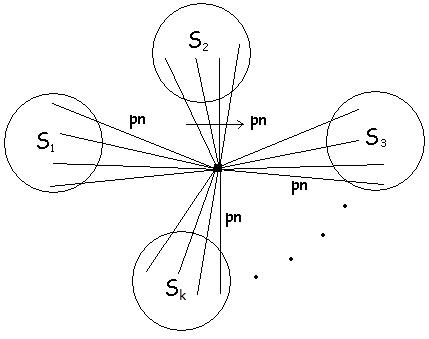
\includegraphics[scale=0.8]{minmaxcounter.JPG}
\caption{$k$-partition can have sparsity much larger than $\Omega(\sqrt{\lambda_k} \polylog k)$ }
\label{fig:minmaxcounter}
\end{figure}

%\begin{lemma}
%\label{lem:minmaxcounter}
%For the graph $G$ in \prettyref{fig:minmaxcounter},
%and for any $k$-partition $S_1, \ldots, S_k$ of its vertex set,
%\[\frac{\max_i \phi_G(S_i)  }{\sqrt{ \lambda_k}} = \Theta \left( \frac{k^2}{\sqrt{n}} \right) \mper \]
%\end{lemma}
%
\begin{proof} (Proof of \prettyref{thm:partition})
In \prettyref{fig:minmaxcounter}, $\forall i \in [k]$, $S_i$ is a clique of size $(n-1)/k$ (pick $n$ so that $k|(n-1)$).
There is an edge from central vertex $v$ to every other vertex of weight $pn$. 
Let $\cP' \defeq \set{S_1 \cup \set{v}, S_2, S_3, \ldots, S_k} $.
For $n > k^3$ and a sufficiently small choice of constant $p$, it is easily verified that the optimum $k$-partition is isomorphic
to $\cP'$.
Furthermore, we have
\[ \max_{S_i \in \cP'} \phi_G(S_i) = \phi_G(S_1 \cup \set{v}) =
	\frac{pn(k-1)}{ \left( \frac{n-1}{k} \right)^2 + pnk}  = \Theta \left(\frac{pk^3}{n} \right) \]
Applying \prettyref{prop:lower} to $S_1, \ldots, S_k$,
we get that 
$$\lambda_k \leq  2\max_i \phi_G(S_i) = \frac{2pn}{
	\binom{(n-1)/k}{2}+ pn} =  \bigO(p k^2/n) \mper $$
Picking $k = n^{1/3}/2$ and a sufficiently small constant for $p$, we have
that for every $k$-partition $T_1, \ldots, T_k$ of the vertex set, 
$$\max_i \phi(T_i) \geq \sqrt{\lambda_k} \cdot
\Omega\left(\frac{k^2}{n^{1/2}}\right) \geq \sqrt{\lambda_k} \cdot
\Omega(\sqrt{k}) $$
\end{proof}


%\Pnote{where is proof of \prettyref{thm:partition}}
%\begin{proof} (Proof of \prettyref{thm:partition})
%Choosing $p$ to be some absolute constant and $k$ between  $n^{1/4} < k < n^{1/3}$ in  
% \prettyref{lem:minmaxcounter} shows that for any $k$-partition $S_1, \ldots, S_k$ of the vertex set, 
%$$\max_i \phi(S_i) \gg \sqrt{\lambda_k} \min\left(\right)$$
%
%\end{proof}


%\begin{remark}
% \prettyref{lem:minmaxcounter} can also be proved for a graph obtained from a star
%graph by adding appropriate weight of self loops. 
%However, in such a graph $k \approx n$, and hence might not be very insightful.
%\end{remark}


\bibliography{bibfile}
\bibliographystyle{amsalpha}




\end{document}


%%%%%%%%%%%%%%%%%%%%%%%%%%%%%%%%%%%%%%%% END OF FILE %%%%%%%%%%%%%%%%%%%%%%%%%%%%%%%%%%%%%%%%%%%%


\section{Sparsest $k$-partition}

\subsection{Recursive partitioning algorithm}
We propose the following recursive algorithm for finding a $k$-partitioning of $G$.
Use the second eigenvector of $\cL$ to find a sparse cut $(C,\bar{C})$. Let $G' = (V,E')$ be the graph
obtained by removing the edges in the cut $(C,\bar{C})$ from $G$ and adding self loops at the endpoints of the edges
removed. Let $\cL'$ be the normalized Laplacian of the graph obtained.
The matrix $\cL'$ is block-diagonal with two blocks for the two components of $G'$.
The spectrum of $\cL'$ (eigenvalues, eigenvectors) is the union of the spectra
of the two blocks. The first two eigenvalues of $\cL'$ are now $0$ and
we use the third largest eigenvector of $\cL'$ to find a sparse cut in $G'$. This is the second eigenvector
in one of the two blocks and partitions that block. We repeat the above process
till we have at least $k$ connected components. This can be viewed as a recursive algorithm, where at each step
one of the current components is partitioned into two; the component partitioned is the one that has the lowest
second eigenvalue among all the current components. The precise algorithm appears in  \prettyref{fig:partition}.

\begin{figure}[ht]
%\begin{tabularx}{\textwidth}{|X|}

\fbox{\parbox{6in}{

\begin{enumerate}
	\item Input : Graph $G=(V,E)$, $m$ such that $1< k < \Abs{V}$
	%\item Initialize : $S = V$
	\item Initialize $i := 2$, and $G_i = G$, $\cL_i = $ normalized Laplacian matrix of $G_i$	

	\begin{enumerate}
		\item Find a sparse cut $(C_i,\bar{C_i})$ in $G_i$ using the $i^{th}$ eigenvector of $\cL_i$
			(the first $i-1$ are all equal to 0).
		\item Let $G_{i+1} := \left( G_i \backslash E_{G_i}(C,\bar{C}) \right) \cup \set{ \set{v,v} :\ \exists\ u \textrm{ such that}
				\set{u,v} \in E_{G_i}(C,\bar{C})   } $ with $w(\set{v,v}) = \sum_{\set{u,v} \in E_{G_i}(C,\bar{C})} w(\set{u,v})$.
		\item If $i=k$ then output the connected components of $G_{i+1}$ and {\sf End} else
		\item Let $\cL_{i+1}$ be the normalized Laplacian matrix of $G_{i+1}$.
			
	\end{enumerate}

\end{enumerate}

}}
%\end{tabularx}
\caption{The Recursive $k$-partition Algorithm}
\label{fig:partition}
\end{figure}



\subsection{Analysis}

In this section, we analyze the recursive partitioning algorithm given
in \prettyref{fig:partition}. Our analysis will also be a
proof of \prettyref{thm:kparts}.  We begin with some monotonicity properties of eigenvalues.

\paragraph{Monotonicity of Eigenvalues.}
In this section we collect some useful properties about the behavior of eigenvalues upon deleting edges and
merging vertices.

\begin{lemma}[Weyl's Inequality]
\label{lem:weyl}
Given a Hermitian matrix $B$ with eigenvalues $\lambda_1 \leq \lambda_2 \leq \ldots \leq \lambda_n$,
and a positive semidefinite matrix $E$, if $\lambda_1' \leq \lambda_2'
\leq \ldots \leq \lambda_n'$ denote the eigenvalues of $B' \defeq
B-E$, then $\lambda_i' \leq \lambda_i$.
\end{lemma}
\begin{proof}
The $i^{th}$ eigenvalue of $B'$ can be written as
\begin{eqnarray*}
\lambda_i' &=& \max_{S: rank(S) = i}\min_{x \in S} \frac{x^TB'x}{x^Tx}\\
           &=& \max_{S: rank(S) = i}\min_{x \in S} \frac{x^TBx - x^TEx}{x^Tx} \\
           &\leq& \max_{S: rank(S) = i}\min_{x \in S} \frac{x^TBx}{x^Tx}\\
           &=& \lambda_i.
\end{eqnarray*}
\end{proof}




\begin{lemma}
\label{lem:weylcut}
Let $\cL$ be the normalized Laplacian matrix of the graph $G$. Let $F$ be any subset of
edges of $G$. For every pair $(i,j) \in F$, remove the edge $(i,j)$ from $G$ and add self
loops at $i$ and $j$ to get the graph $G'$. Let $\cL'$ be the normalized Laplacian
matrix of $G'$. Let the eigenvalues of $\cL$ be $0 \leq \lambda_2 \leq \ldots \leq \lambda_n$ and
let the eigenvalues of $\cL'$ be $0 \leq \lambda_2'\leq \lambda_3'\leq \ldots \leq \lambda_n'$.
Then $\lambda_i' \leq \lambda_i$ $\forall i \in [n]$.
\end{lemma}



\begin{proof}

Let $C \defeq \cL - \cL'$ is the matrix corresponding to the edge subset $F$. It has non-negative entries along its diagonal
and non-positive entries elsewhere such that $\forall i$ $c_{ii} = - \sum_{ j \neq i} c_{ij} $.
$C$ is symmetric and positive semi-definite as for any vector $x$ of appropriate
dimension, we have
\[
x^T C x =  \sum_{ij} c_{ij} x_i x_j =
-\frac{1}{2} \sum_{i \neq j} c_{ij}(x_i - x_j)^2 \geq 0.
\]

Using \prettyref{lem:weyl}, we get that $\lambda_i' \leq \lambda_i$  $\forall i \in [n]$.
\end{proof}
\prettyref{lem:weylcut} shows that the eigenvalues of $\cL_{i}$ are monotonically non-increasing with $i$.
This will show that $\phi_{G_i}(C_i) \leq \sqrt{2 \lambda_k}$.
We are now ready to prove Theorem \ref{thm:kparts}.

\begin{proof}[Proof of Theorem \ref{thm:kparts} ]
Let $\cP$ be the partition output by the algorithm and let $S(\cP)$ denote the sum of weights of the
smallest $k-1$ pieces in $\cP$.
Note that we need only the smaller side of a cut to bound the size of the cut : $w(E_G(S,\bar{S})) \leq \phi_G \ w(S)$.
We define the notion of a $\ct$ $T = (V(T),E(T))$ as follows:
$V(T) = \set{V} \cup \set{C_i : i \in [k]}$
(For any cut $(C_i,\bar{C_i})$ we denote the part with the smaller weight by $C_i$ and the part with the
larger weight by $\bar{C_i}$. We break ties arbitrarily).
We put an edge between $S_1, S_2 \in V(T)$ if $\not\exists S \in V(T)$ such that
$S_1 \subsetneq S \subsetneq S_2$ or $S_2 \subsetneq S \subsetneq S_1$,
(one can view $S_1$ as a 'top level' cut of $S_2$ in the former case).

Clearly, $T$ is connected and is a tree. We call $V$ the root of $T$.
We define the {\em level} of a node in $T$ to be its depth from the root.
We denote the level of node $S \in V(T)$ by $L(S)$.
The root is defined to be at level $0$.
Observe that $S_1 \in V(T)$ is a descendant of $S_2 \in V(T)$ if and only if
$S_1 \subsetneq S_2$.
Now $\edges(\cP) = \cup_i E_{G_i}(C_i,\bar{C_i}) = \cup_i \cup_{j : L(C_j) = i} E_{G_j}(C_j,\bar{C_j})$.
We make the following claim.



\begin{Claim}
\label{claim:leveli}
\[ w(\cup_{ j : L(C_j) = i} E(C_j,\bar{C_j})) \leq 2 \sqrt{ \lambda_k} \ S({\cP}) \]
\end{Claim}

\begin{proof}
By definition of level, if $L(C_i) = L(C_j)$, $i \neq j$, then the node corresponding to
$C_i$ in the $T$ can not be an ancestor or a descendant of the node corresponding to
$C_j$. Hence, $C_i \cap C_j = \phi$.
Therefore, all the sets of vertices in level $i$ are pairwise disjoint. Using Cheeger's inequality
we get that $E(C_j,\bar{C_j}) \leq 2\sqrt{ \lambda_k}  w(C_j)$. Therefore
\[  w(\cup_{ j : L(C_j) = i} E(C_j,\bar{C_j})) \leq 2 \sqrt{ \lambda_k} \sum_{ j : L(C_j) = i} w(C_j) \leq 2 \sqrt{ \lambda_k}  S({\cP})\]


\end{proof}

\noindent
This claim implies that $\phi(\cP) \leq 2 \sqrt{\lambda_k} \ {\sf height}(T)$.

\noindent
The height of $T$ might be as much as $k$. But we will show that we can assume height($T$)
to be $\log k$. For any path in the tree $v_1,v_2, \ldots, v_{p-1}, v_p$ such that {\sf deg}$(v_1) > 2$,
${\sf deg}(v_i) = 2$ (i.e. $v_i$ has only 1 child in $T$) for $1 < i < k$, we have $w(C_{v_{i+1}}) \leq w(C_{v_i})/2 $, as ${v_{i+1}}$ being
a child of ${v_i}$ in the $T$ implies that $C_{v_{i+1}}$ was obtained by cutting $C_{v_{i}}$ using it's
second eigenvector. Thus
$\sum_{i=2}^p w(C_{v_i}) \leq w(C_{v_1})$. Hence we can modify the $T$ as follows : make the nodes $v_3,\ldots,v_p$
children of $v_2$. The nodes $v_3,\ldots,v_{p-1}$ now  become leaves whereas the subtree rooted at $v_p$ remains unchanged.
We also assign the level of each node as its new distance from the root.
In this process we might have destroyed the property that a node is obtained from by cutting its parent, but we have the property
that $ w(\cup_{j : L(C_j) = i} E(C_j,\bar{C_j})) \leq 4 \sqrt{\lambda_k}  S({\cP})$ $\forall i$.

\begin{Claim}
\[ w(\cup_{ j : L(C_j) = i} E(C_j,\bar{C_j})) \leq 4 \sqrt{ \lambda_k} \ S({\cP}) \]

\end{Claim}

\begin{proof}
If the nodes in level $i$ are unchanged by this process, then the claim clearly holds. If
any node $v_j$ in level $i$ moved to a higher level, then the nodes replacing $v_j$ in level $i$
would be descendants of $v_j$ in the original $T$ and hence would have weight at most $w(C_{v_j})$.
If the descendants of some node $v_j$ got added to level $i$, then, as seen above, their combined
weight would be at most $w(C_{v_{j}})$. Hence,

\[  w(\cup_{ j : L(C_j) = i} E(C_j,\bar{C_j})) \leq 2 \left(  2 \sqrt{\lambda_k}  \sum_{ j : L(C_j) = i} w(C_j) \right) \leq 4 \sqrt{\lambda_k} \ S({\cP}) \].

\end{proof}

\noindent

Repeating this process we can ensure that no two adjacent nodes in the $T$ have degree 2.
Hence, there are at most $ \log k$ vertices along any path starting from the root which have exactly
one child.
Thus the height of the new $\ct$ is at most $2 \log k$. Thus $\edges(\cP) \leq 8 \sqrt{ \lambda_k} \log k \ S({\cP}) $
and hence $\phis \leq \frac{\edges(\cP)}{S({\cP})} \leq 8 \sqrt{\lambda_k} \log k  $.

\end{proof}


\section{Gap examples}
In this section, we present constructions of graphs that serve as
lower-bounds against natural classes of algorithms.  We begin with a
family of graphs on which the performance of recursive partitioning
algorithms is poor for the $k$-Sparse cuts problem. 


\subsection{Recursive Algorithms}
\label{badrecursive}

Recursive algorithms are one of most commonly used techniques in practice for graph multi-partitioning.
However, we show that partitioning a graph into $k$ pieces using a simple recursive algorithm can yield as many
as $k(1-o(1))$ sets with expansion much larger than $\sqrt{\lambda_k} {\sf polylog} k$.
Thus this is not an effective method for finding many sparse cuts.

The following construction (Figure \ref{fig:verybadrecursive}) shows that the partition of $V$ obtained
using the recursive algorithm in Figure \ref{fig:partition}
can give as many as $k(1 - o(1))$ sets that have expansion $\Omega(1)$ while $\lambda_k \leq \bigO(k^2/n^2)$.

\begin{figure}[htp]
\centering
\includegraphics[scale=0.8]{verybadrecursive.jpg}
\caption{Recursive algorithm can give many sets with very small expansion}
\label{fig:verybadrecursive}
\end{figure}


In this graph, there are $p \defeq k^{\e}$ sets $S_i$ for $1 \leq i \leq k^{\e}$.
We will fix the value of $\e$ later.
Each of the $S_i$ has
$k^{1 - \e}$ cliques $\set{S_{ij} :   1 \leq j \leq k^{1 -\e}}$  of size $n/k$ which are sparsely connected
to each other. The total weight of the edges from $S_{ij}$ to $S_i \backslash S_{ij}$ is equal to a constant
$c$.
In addition to this, there are also $k - k^{\e}$ vertices $v_i : 1 \leq i \leq k - k^{\e}$. The weight of edges
from $S_i$ to $v_j$ is equal to $k^{-\e}$.


\begin{Claim}
\begin{enumerate}
\item $\phi(S_{ij}) \leq  (c+1) k^2/n^2$ $\forall i,j $
\item $\phi(S_i) \leq 1/(c+1) \phi(S_{ij})$ $\forall i,j$
\item $\lambda_k = \bigO(k^2/n^2)$

\end{enumerate}
\end{Claim}


\begin{proof}
\begin{enumerate}
\item \[ \phi(S_{ij}) =   \frac{c + \frac{(k - k^{\e}) k^{-\e}}{k^{1 - \e}}}{ (\frac{n}{k})^2 + c + \frac{(k - k^{\e}) k^{-\e}}{k^{1 - \e}}  }  \leq
\frac{(c+1) k^2}{n^2} \]
\item $w(S_i) = \sum_j w(S_{ij})$, but for each $S_{ij}$ only $1/(c+1)$ fraction of edges incident at $S_{ij}$
are also incident at $S_i$. Therefore, $\phi(S_i) \leq 1/(c+1) \phi(S_{ij})$.

\item Follows from $(1)$ and  \prettyref{prop:lower}.

\end{enumerate}
\end{proof}


For appropriate values of $\e$ and $k$,  the partition output by the recursive algorithm will be
$\set{S_i : i \in [k^{\e}]} \cup \set{v_i : i \in [k - k^{\e}]}$. Hence, $k(1 - o(1))$ sets have
expansion equal to $1$.


